%% 
%% Copyright 2007-2025 Elsevier Ltd
%% 
%% This file is part of the 'Elsarticle Bundle'.
%% ---------------------------------------------
%% 
%% It may be distributed under the conditions of the LaTeX Project Public
%% License, either version 1.3 of this license or (at your option) any
%% later version.  The latest version of this license is in
%%    http://www.latex-project.org/lppl.txt
%% and version 1.3 or later is part of all distributions of LaTeX
%% version 1999/12/01 or later.
%% 
%% The list of all files belonging to the 'Elsarticle Bundle' is
%% given in the file `manifest.txt'.
%% 
%% Template article for Elsevier's document class `elsarticle'
%% with harvard style bibliographic references

\documentclass[preprint,12pt,authoryear]{elsarticle}

%% Use the option review to obtain double line spacing
%% \documentclass[authoryear,preprint,review,12pt]{elsarticle}

%% Use the options 1p,twocolumn; 3p; 3p,twocolumn; 5p; or 5p,twocolumn
%% for a journal layout:
%% \documentclass[final,1p,times,authoryear]{elsarticle}
%% \documentclass[final,1p,times,twocolumn,authoryear]{elsarticle}
%% \documentclass[final,3p,times,authoryear]{elsarticle}
%% \documentclass[final,3p,times,twocolumn,authoryear]{elsarticle}
%% \documentclass[final,5p,times,authoryear]{elsarticle}
%% \documentclass[final,5p,times,twocolumn,authoryear]{elsarticle}

%% For including figures, graphicx.sty has been loaded in
%% elsarticle.cls. If you prefer to use the old commands
%% please give \usepackage{epsfig}

%% The amssymb package provides various useful mathematical symbols
\usepackage{amssymb}
%% The amsmath package provides various useful equation environments.
\usepackage{amsmath}
\biboptions{authoryear}
\usepackage{booktabs}
\usepackage{caption}
\usepackage{graphicx}
\graphicspath{{figures/}}
\usepackage{placeins}
\usepackage{tabularx}
\usepackage{array}
\usepackage{ragged2e}
\usepackage{float}

\newcolumntype{P}[1]{>{\RaggedRight\arraybackslash\hspace{0pt}}p{#1}}
\newcolumntype{Y}{>{\RaggedRight\arraybackslash}X}



%% The amsthm package provides extended theorem environments
%% \usepackage{amsthm}

%% The lineno packages adds line numbers. Start line numbering with
%% \begin{linenumbers}, end it with \end{linenumbers}. Or switch it on
%% for the whole article with \linenumbers.
%% \usepackage{lineno}

\journal{International Journal of Pharmaceutics}

\begin{document}

\begin{frontmatter}
%\begin{graphicalabstract}
%%\includegraphics[width=\textwidth,height=0.6\textheight,keepaspectratio]{GraphicalAbstract}
%\end{graphicalabstract}
%\title{Diagnosing Predictability Limits in Literature-Mined PLGA Microparticle Drug Release Data}

%% Authors
\author[aff1]{Kushaan Sharma\corref{cor1}}
\ead{kushaan.s2007@utexas.edu} % <-- replace if different email

\author[aff2]{Aryan Shah}
\author[aff3]{Syna Sharma}

\cortext[cor1]{Corresponding author}

%% Affiliations
\affiliation[aff1]{
  organization={The University of Texas at Austin},
  addressline={2515 Speedway},
  city={Austin},
  state={TX},
  postcode={78712},
  country={USA}
}

\affiliation[aff2]{
  organization={Texas A\&M University},
  addressline={400 Bizzell St},
  city={College Station},
  state={TX},
  postcode={77840},
  country={USA}
}

\affiliation[aff3]{
  organization={University of the Incarnate Word School of Osteopathic Medicine},
  addressline={7615 Kennedy Hill Dr},
  city={San Antonio},
  state={TX},
  postcode={78235},
  country={USA}
}




\begin{abstract}
PLGA microparticles are widely used for sustained drug delivery, yet published in vitro release profiles remain difficult to predict quantitatively across studies. Here we curate and standardize a literature-mined dataset of PLGA microparticle formulations measured under comparable in vitro conditions and use machine learning in combination with mechanistic, interpretable targets to diagnose the attainable predictability from commonly reported variables. We parameterize early-time release using Korsmeyer--Peppas descriptors and quantify 24-hour burst behavior, then evaluate model performance under grouped cross-validation and applicability-domain analysis. Across 278 formulations meeting completeness criteria, grouped cross-validation yielded a global predictive performance of $R^2 \approx 0.42$. Augmenting the feature space with formulation-method metadata produced only marginal improvement, and predictive consistency across model families was preserved. These results evaluate whether predictive performance exhibits an apparent ceiling imposed by current reporting practices rather than model choice, indicating an information-limited rather than algorithm-limited regime. The findings motivate concrete reporting priorities for the field and define a reliability-oriented pathway for data-driven screening in PLGA formulation development.
\end{abstract}

\begin{highlights}
\item Compiled 321 PLGA microparticle formulations from 113 studies; standard conditions.
\item Mechanistic parameters (Peppas n and K) show only limited predictability ($R^2 \approx 0.42$).
\item Performance drops in leave-one-study-out tests, showing strong study-level effects.
\item Early 24 h burst cannot be reliably predicted and is high across most studies.
\item Reporting-gap analysis identifies missing variables and proposes a new checklist.
\end{highlights}

\begin{keyword}
PLGA microparticles \sep drug release \sep burst release \sep machine learning \sep applicability domain \sep Korsmeyer--Peppas
\end{keyword}

\end{frontmatter}

\section{Introduction}

Poly(lactic-co-glycolic acid) (PLGA) microparticles are among the most widely studied biodegradable carriers for sustained drug delivery and have become a foundational platform in controlled-release formulation research \citep{MakadiaSiegel2011,FreibergZhu2004}. The appeal of PLGA systems stems from their biodegradability and tunable release behavior, which can reduce dosing frequency and help maintain therapeutic exposure over extended periods \citep{MakadiaSiegel2011,Fredenberg2011}. Despite this maturity, formulation development for PLGA microparticles remains heavily empirical because drug release is shaped by multiple coupled factors that vary across laboratories and manufacturing routes \citep{Fredenberg2011,Jain2000}. As a result, ostensibly similar PLGA systems can exhibit substantially different release profiles, complicating translation and slowing rational design \citep{Fredenberg2011}.

Mechanistically, release from PLGA matrices reflects an interplay of drug diffusion, polymer hydration and degradation, pore formation, and erosion, with the relative contributions evolving over time \citep{Fredenberg2011}. Polymer composition (e.g., lactic:glycolic ratio), molecular weight, and end-group chemistry influence water uptake and hydrolysis kinetics, which in turn modulate microstructure development and release rates \citep{MakadiaSiegel2011,Fredenberg2011}. In parallel, micro- and meso-scale morphology, including particle size, porosity, and drug spatial distribution, strongly impacts early-time release and the transition to degradation-controlled regimes \citep{Fredenberg2011}. Critically, many of these morphological attributes are not independent material properties: they are created during manufacturing. Common preparation methods (e.g., emulsion-based routes) can yield different internal structures depending on solvent choice, surfactant conditions, mixing and emulsification energy, and solvent removal dynamics \citep{Jain2000}. Consequently, process parameters can act as dominant drivers of between-study variability, particularly when they are not reported in a standardized way \citep{Jain2000,Fredenberg2011}.

A particularly important manifestation of this variability is \emph{burst release}, the rapid early-time liberation of a fraction of drug that is often associated with surface-localized payload and connected pore networks \citep{Yoo2020Burst}. Burst behavior is frequently treated as a critical quality attribute in PLGA microparticle development because it can shape initial exposure and safety margins, even when long-term release remains acceptable \citep{Yoo2020Burst,ICHQ8R2}. Yet burst is also highly sensitive to formulation microstructure and measurement conditions, making it challenging to compare across studies without careful standardization \citep{Yoo2020Burst,Fredenberg2011}. Even the \emph{in vitro} release protocol can measurably influence the observed profile; for example, maintaining perfect sink conditions may alter PLGA degradation behavior and thereby affect release kinetics \citep{Klose2011Sink}. These experimental dependencies connect directly to broader challenges in establishing robust in vitro--in vivo relationships for complex non-oral drug products \citep{ShenBurgess2015}.

To manage complexity and improve interpretability, PLGA release is often summarized using mechanistic or semi-empirical models. In the early-time regime, the Korsmeyer--Peppas power law is widely used to compactly describe release behavior and to provide parameters that can be compared across systems within a defined validity window \citep{Korsmeyer1983,RitgerPeppas1987}. While PLGA release can involve multiple overlapping physical processes, parameterized targets can be useful in practice because they translate heterogeneous time-series curves into a small set of interpretable descriptors \citep{Fredenberg2011}. Such targets can also support decision-making consistent with quality-by-design (QbD) frameworks, where the goal is not only prediction but also identification of controllable drivers and risk-relevant regimes \citep{ICHQ8R2}.

In parallel, machine learning (ML) is increasingly used to accelerate formulation development by learning nonlinear relationships between composition, process, and performance from experimental data \citep{Bannigan2021}. When datasets are information-rich and generated under standardized protocols, ML models have demonstrated utility for polymeric long-acting injectables and related controlled-release systems \citep{Bannigan2023LAI}. In this context, predictive accuracy itself is not the primary objective; rather, model behavior is used to interrogate the information content of reported formulation variables. Recent perspective work has also highlighted how ML could help navigate the design space and development bottlenecks for polymer microparticles in long-acting injectable contexts \citep{Bao2025IJP}. However, a key failure mode arises when models are trained on literature-mined corpora: the published record often omits or inconsistently reports critical process variables that determine microstructure (and therefore release), creating latent confounders that cap achievable performance \citep{Jain2000,Fredenberg2011}. In this setting, predictive performance may plateau at a finite level: models can capture reproducible structure, yet additional algorithmic complexity fails to substantially improve accuracy because the available covariates incompletely describe the microstructure-defining processes. Thus, limited performance does not imply that PLGA release is inherently unpredictable, but rather that the published feature space may be insufficient to support fully quantitative prediction.


This motivates a shift in how ML is used on literature-mined PLGA release data. Rather than treating model performance as the final objective, ML can be used as an \emph{instrument} to diagnose the limits of predictability imposed by reporting practices and study heterogeneity. A complementary concept from quantitative structure--activity relationship (QSAR) modeling is the \emph{applicability domain} (AD), which characterizes where a model is expected to be reliable based on the similarity of new points to the training data \citep{OECD2004QSAR,Netzeva2005AD}. In practice, leverage-based diagnostics (often visualized via Williams plots) are a common approach to flag potentially out-of-domain predictions and interpret residual behavior \citep{WeaverGleeson2008}. In heterogeneous, literature-mined datasets, AD analysis can also be viewed as a map of the data manifold: it can test for subdomains where the literature is internally consistent enough to support stronger learning, even if global prediction remains limited \citep{Netzeva2005AD,WeaverGleeson2008}.

In this work, we curate and standardize a literature-mined dataset of PLGA microparticle release profiles measured under comparable \emph{in vitro} conditions to quantify the attainable predictive ceiling from commonly reported variables. We parameterize early-time release using Korsmeyer--Peppas descriptors \citep{Korsmeyer1983,RitgerPeppas1987} and quantify 24-hour burst behavior \citep{Yoo2020Burst}, then evaluate prediction under grouped validation to avoid within-formulation leakage. Finally, we apply applicability-domain analysis to partition the dataset and to assess the uniformity of model reliability across the domain \citep{OECD2004QSAR,WeaverGleeson2008,Netzeva2005AD}. By framing ML as a diagnostic tool for the information content of the published record, the study provides concrete guidance on which experimental and process variables should be reported more consistently to improve predictability and to support risk-focused screening aligned with QbD principles \citep{ICHQ8R2}.

%% --- Add your remaining sections here ---
%========================
\section{Materials and methods}

\subsection{Literature-derived dataset and scope}
A structured dataset of poly(lactic-\emph{co}-glycolic acid) (PLGA) microparticle drug-release profiles and formulation descriptors was assembled from a systematic literature review. In total, 1{,}231 records were screened and 113 studies (unique DOIs) were included, yielding 321 unique formulations across 89 drugs and 4{,}913 release observations (5--48 time points per formulation; average $\sim$15). Each release observation corresponds to a single row indexed by a \textit{Formulation Index} and a sampling time (\texttt{Time}), with an associated cumulative release value (\texttt{Release}).

The dataset focuses on stand-alone PLGA microparticles/microspheres with an \textit{in vitro} cumulative release curve (minimum five reported time points), known drug identity (including SMILES for descriptor computation), and sufficient formulation metadata (e.g., polymer molecular weight, LA:GA ratio, particle size, loading/encapsulation). Studies were excluded when release was reported only \textit{in vivo}, when systems were composite/hybrid dosage forms (e.g., hydrogels, scaffolds, implants) with confounded mechanisms, or when key formulation fields were not reported. The overarching goal is to evaluate how well machine-learning models generalize across heterogeneous, multi-source literature data and to quantify the attainable predictive ceiling and its robustness to feature augmentation \citep{ICHQ8R2,Bannigan2021,Bannigan2023LAI,Bao2025IJP}.Of the 321 curated formulations, 278 met completeness requirements for the primary modeling feature set after removal of samples with missing essential descriptors. All predictive analyses therefore report performance on this modeling subset (N = 278), while the full dataset is retained for reporting-gap statistics.


\subsection{Release-curve extraction and digitization uncertainty}
Release profiles were collected from the primary literature as discrete (time, release) pairs. The majority of curves were digitized from published release-profile figures using WebPlotDigitizer (v4.x) \citep{Rohatgi2022WebPlotDigitizer}, with a small minority extracted from tabular or supplementary numerical data when available. No explicit digitization-error propagation (e.g., repeated digitization trials or uncertainty bands) was performed; digitization/transcription uncertainty is therefore treated as a component of the expected experimental heterogeneity in literature systems.

To reduce sensitivity to irregular sampling and to support consistent downstream target estimation, release curves were optionally resampled using monotone piecewise cubic Hermite interpolation (PCHIP), which preserves curve shape and monotonicity while generating uniformly sampled trajectories \citep{FritschCarlson1980,Virtanen2020SciPy}. Basic curve-level quality control excluded formulations with fewer than five sampled time points (insufficient resolution for stable kinetic estimation; Section~\ref{subsec:targets}) and removed physically implausible mechanistic fits (e.g., Korsmeyer--Peppas exponents outside $0 \le n \le 2$). Importantly, the observed prediction errors substantially exceed reported digitization uncertainty in comparable extraction studies \citep{Drevon2017WPD}, indicating that inter-study variability (manufacturing and reporting heterogeneity) rather than graphical extraction error dominates the effective noise floor in this heterogeneous literature compilation \citep{Fredenberg2011,FreibergZhu2004}.

\subsection{Definition of a unique formulation and leakage-free grouping}
\label{subsec:formulation_index}
A \textit{unique formulation} is defined as a single distinct value of \texttt{Formulation Index}, corresponding to one reported formulation instance (i.e., a unique combination of drug and key formulation attributes from a single source study). All time points sharing the same index are treated as a single release curve. To prevent temporal leakage (multiple time points from the same curve appearing in both training and test sets), all validation and holdout splitting are performed using group-based strategies where \texttt{Formulation Index} is the grouping variable \citep{Roberts2017CVStructure}. Thus, each formulation is confined to a single fold, ensuring that evaluation reflects generalization to entirely unseen formulations rather than interpolation over additional time points from known curves. For learning tasks where targets are formulation-level quantities (Peppas $n$, Peppas $K$, and \texttt{Burst\_24h}), the fitted target value for a given formulation is assigned to each release observation row associated with that \texttt{Formulation Index}; all splitting remains grouped by \texttt{Formulation Index} to prevent leakage while retaining the long-format structure of the digitized dataset.

\subsection{Unit conventions and standardization}
\label{subsec:units}
\subsubsection{Time axis and burst definition}
Release curves record \texttt{Time} as reported in the source study and \texttt{Release} as a fraction (0--1; slight overshoot above 1 can occur in reported cumulative data). For burst analysis, \texttt{Burst\_24h} is defined as cumulative release at 24 hours and is obtained by one-dimensional interpolation at the 24-hour mark. To ensure consistent interpretation, time values were standardized such that 24 corresponds to 24~h for all burst computations.

\subsubsection{Polymer molecular weight}
Polymer molecular weight is represented by a single numeric feature (\texttt{Polymer MW}) assembled from literature-reported fields with the priority order $M_w$ (weight-average) $\;>\;$ $M_n$ (number-average) $\;>\;$ an unspecified molecular-weight field when neither $M_w$ nor $M_n$ is available. Values are used as reported; any residual heterogeneity in polymer molecular-weight reporting is treated as part of the literature noise floor \citep{Fredenberg2011,MakadiaSiegel2011,Jain2000}.

\subsubsection{LA:GA ratio}
The lactic-to-glycolic ratio is represented as a numeric feature (\texttt{LA/GA}) and used directly as \texttt{LA\_GA\_numeric}. Ratios reported textually in the source literature (e.g., ``50:50'') were converted upstream into a single numeric ratio consistent with this representation.

\subsection{Mechanistic target engineering}
\label{subsec:targets}
\subsubsection{Korsmeyer--Peppas parameterization}
Rather than learning release percentages at arbitrary times, the learning targets were defined as physics-informed parameters from the Korsmeyer--Peppas power-law model \citep{Korsmeyer1983,RitgerPeppas1987}:
\begin{equation}
\frac{M_t}{M_\infty} = K\, t^n,
\end{equation}
where $n$ is the release exponent (mechanistic regime indicator) and $K$ is a rate constant. For each formulation, $n$ and $K$ were estimated using log--log linear regression of $\log(M_t/M_\infty)$ versus $\log(t)$ over the sub-60\% release region ($M_t/M_\infty \le 0.60$) to reduce late-time saturation effects. Basic plausibility constraints were enforced (e.g., discarding nonphysical fits such as $n<0$ or $n>2$). Formulations with fewer than five time points were excluded from mechanistic fitting to reduce unstable parameter estimates.

\subsubsection{Initial burst metric and risk classes}
To address the known sensitivity of early-time release to formulation and processing heterogeneity \citep{Fredenberg2011,Yoo2020Burst,FreibergZhu2004}, \texttt{Burst\_24h} was computed by interpolation at 24~h. In addition to regression on \texttt{Burst\_24h}, a safety-oriented classification task binned formulations into three burst-risk regimes (selected to reflect clinical exposure risk tiers):
\begin{itemize}
  \item Class 0 (Low burst): \texttt{Burst\_24h} $< 10\%$
  \item Class 1 (Intermediate): $10\% \le$ \texttt{Burst\_24h} $< 40\%$
  \item Class 2 (High burst): \texttt{Burst\_24h} $\ge 40\%$
\end{itemize}
No class reweighting, resampling, or synthetic augmentation was applied; the classifier was trained directly on the available labeled formulations. Given the severe class imbalance observed in the compiled literature, classification results were interpreted using class-sensitive metrics rather than accuracy alone \citep{HeGarcia2009Imbalanced,SokolovaLapalme2009Metrics}.

\subsection{Feature engineering and model matrix}
A fixed, purely numeric feature set ($p=15$) was used for all learning tasks (mechanistic parameters and burst regression/classification). Chemical descriptors were computed from drug SMILES using RDKit \citep{RDKitZenodo} (e.g., molecular weight, topological polar surface area, logP-related descriptors, hydrogen-bond counts, and rotatable bonds), and formulation/process descriptors were taken from curated literature fields (e.g., particle size, loading capacity, and encapsulation efficiency).

In addition, a composite \textit{Hydrophilicity Index} was defined as
\begin{equation}
\text{Hydrophilicity Index} = \left(\frac{1}{\text{LA/GA}}\right)\left(\frac{1}{\text{Polymer MW}}\right),
\end{equation}
to provide a monotonic proxy for polymer aqueous accessibility that captures the joint directionality of increased glycolide content (lower LA:GA) and reduced chain length on water penetration and degradation propensity \citep{MakadiaSiegel2011,Fredenberg2011}. This composite descriptor is used only as a directional monotonic encoding, not a physical quantity; rather, it serves as a heuristic feature summarizing two well-established qualitative trends in PLGA behavior \citep{MakadiaSiegel2011,Fredenberg2011}.

\subsection{Formulation-method augmentation}
To test whether predictive performance was limited by omission of high-level process information rather than intrinsic variability, a robustness analysis was performed by augmenting the feature set with a categorical \texttt{Formulation Method} variable. This variable encoded the primary microparticle preparation route reported in the source article (e.g., single emulsion, double emulsion, nanoprecipitation, spray drying) using one-hot encoding within the training folds.

All preprocessing, encoding, and scaling were performed inside cross-validation folds to prevent information leakage. Model architectures, validation splits, and hyperparameters were unchanged from the primary analysis. The objective of this experiment was not to optimize performance but to test whether inclusion of a coarse process descriptor materially altered global predictability.

Improvement limited to marginal changes in $R^2$ was interpreted as evidence that predictive performance is constrained by missing fine-grained structural descriptors rather than omission of high-level formulation categories.


\subsection{Preprocessing, model families, and specification}
To avoid optimistic bias in a heterogeneous, literature-derived dataset, all preprocessing steps (imputation and scaling) were performed within-fold during validation. Missing values were handled exclusively via mean imputation using training data only, and features were standardized using a scaler fit on the training portion of each fold \citep{Pedregosa2011Sklearn}. No missingness-indicator variables were included.

\subsubsection{Model families as probes of learnability}
Regression targets ($n$, $K$, and \texttt{Burst\_24h}) were modeled using a stacked ensemble comprising three base learners: random forests, gradient-boosted trees, and an RBF-kernel support vector regressor, with a linear ridge meta-learner \citep{Breiman2001RF,CortesVapnik1995SVM,HoerlKennard1970Ridge,Wolpert1992Stacked,Chen2016XGBoost}. Hyperparameters were fixed (no grid search or Bayesian tuning) to emphasize interpretability and to quantify information limits under realistic inter-study heterogeneity rather than to optimize benchmark performance. The ensemble was selected to span tree-based, kernel-based, and linear hypothesis classes, allowing predictive consistency across model families to be interpreted as evidence of learnable signal rather than model-specific fitting. If models with different inductive biases converge to similar performance, the limiting factor is information content rather than model capacity.

For benchmarking, we also evaluated baseline model families under the same grouped cross-validation protocol: ordinary least-squares linear regression, a random forest regressor, and gradient-boosted decision trees (XGBoost) \citep{Breiman2001RF,Chen2016XGBoost}. These baselines were used diagnostically to assess whether predictive performance was consistent across structurally distinct hypothesis classes.

Burst-risk classes were predicted using a gradient-boosted tree classifier (XGBoost) with a three-class softmax objective \citep{Chen2016XGBoost}. As above, hyperparameters were fixed by design to preserve the role of the models as analytical probes rather than optimization targets.

\subsection{Validation protocol}
Model performance was assessed using grouped cross-validation, where the grouping variable was \texttt{Formulation Index} (Section~\ref{subsec:formulation_index}). Regression performance was summarized using $R^2$, MAE, and RMSE computed from pooled out-of-fold predictions. A separate grouped holdout split (80/20 by formulation) was used as an additional leakage check for the burst-risk classifier.

To test generalization across laboratories, we additionally performed leave-one-study-out (LOSO) validation at the DOI level: each iteration held out one entire study, trained the stacked ensemble on the remaining studies, and evaluated on the held-out DOI. Regression performance under LOSO was reported using pooled $R^2$, MAE, and RMSE across all held-out studies.

For burst-risk classification, performance was summarized using the confusion matrix, per-class precision and recall, and macro-averaged F1 (Macro-F1), computed from grouped predictions to avoid within-formulation leakage \citep{HeGarcia2009Imbalanced,SokolovaLapalme2009Metrics}.

\subsection{Variance decomposition by study identity (ICC-1)}
To quantify the proportion of variance attributable to study-level effects (proxies for laboratory-specific processing differences), we performed a one-way random-effects analysis (ICC-1) on studies contributing at least two formulations. For each target ($n$, $K$, and \texttt{Burst\_24h}), variance components were estimated using a one-way random-effects model, yielding $\sigma^2_{\text{between}}$ and $\sigma^2_{\text{within}}$. ICC(1) was computed as
\begin{equation}
\mathrm{ICC}(1) = \frac{\sigma^2_{\text{between}}}{\sigma^2_{\text{between}} + \sigma^2_{\text{within}}}
\end{equation}
and inference followed standard ICC formulations for one-way random-effects designs \citep{ShroutFleiss1979ICC,McGrawWong1996ICCInference}. An ANOVA $F$-test was used to assess whether between-study variability exceeded within-study variability, and results were reported for the subset of studies meeting the minimum formulation-count criterion.

\subsection{Applicability domain and uncertainty quantification}
\label{sec:ad_uq}
Given the risk of extrapolation in QSAR and QSPR style modeling on heterogeneous chemical space, applicability-domain (AD) analysis was used to separate ``in-domain'' predictions from high-leverage extrapolations \citep{OECD2004QSAR,OECD2007QSARGuidance,WeaverGleeson2008,Netzeva2005AD,Tropsha2010BestPracticesQSAR,Gramatica2007QSARValidation}. Leverage values were computed from the scaled design matrix, and a warning leverage threshold $h^*$ was used to flag extrapolative points (Williams-plot analysis). Performance was reported separately for formulations inside and outside the warning leverage region to test whether the AD behaves as a monotone safety filter or instead reveals heterogeneous islands of predictability across literature sub-domains \citep{WeaverGleeson2008,Netzeva2005AD}.

Prediction uncertainty was quantified using an ensemble-disagreement proxy: for each sample, the uncertainty score was defined as the standard deviation of the base-learner predictions within the stacked model. This uncertainty was not calibrated to probabilistic coverage; it was used diagnostically to test whether error increases with model disagreement, consistent with the study emphasis on reliability over headline accuracy \citep{WeaverGleeson2008}.

\subsection{Reporting-gap analysis and feature importance}
To relate predictive performance to literature reporting practices, we quantified variable availability across the compiled studies and compared it against predictive importance and mechanistic relevance. Availability percentages were computed at the formulation level after harmonization of synonymous reporting fields. In particular, polymer molecular weight was represented as a composite feature using the priority order $M_w > M_n >$ unspecified molecular weight; if multiple molecular-weight fields appeared within a study, the harmonized value followed this priority rule. Mechanistic relevance was grounded in established PLGA release pathways and the known sensitivity of early release to microstructure and processing conditions \citep{Fredenberg2011,FreibergZhu2004,Jain2000,Yoo2020Burst,KloseSiepmann2006Porosity}.

Feature importance values for prediction of the release exponent $n$ were derived from a random forest regressor using standard impurity-based importance scores (mean decrease in impurity) \citep{Breiman2001RF}. Importance values were computed on grouped cross-validation training folds and summarized as average percent contribution across features; only features exceeding a 5\% importance threshold were reported.

Mechanistically relevant but unreported process variables (e.g., internal porosity, solvent removal rate, stirring/homogenization parameters, and polymer end-group chemistry) were identified from established PLGA release mechanisms and recorded as absent when not quantitatively specified in the source articles \citep{Fredenberg2011,FreibergZhu2004,Jain2000,KloseSiepmann2006Porosity,Yoo2020Burst}.

\section{Results and Discussion}

\subsection{Dataset Overview and Feature Summary}

We assembled a dataset of 321 unique PLGA microparticle formulations by synthesizing data from 113 primary studies. This effort yielded a total of 4,913 release measurements across 89 different drugs, utilizing specialized digitization tools to extract high-fidelity numerical data from graphical literature sources. We noted significant variation in how much data each study provided; individual formulations contributed anywhere from 5 to 48 time points, averaging roughly 15 per curve. This raw data was then structured into a fixed design matrix consisting of 15 numerical covariates.

To characterize the drugs, we used RDKit to derive six descriptors from SMILES strings---specifically molecular weight, lipophilicity, topological polar surface area, rotatable bonds, and hydrogen-bond counts. We supplemented these with three additional drug properties as reported in the original source papers. The remaining six features in our matrix describe the physical formulation and process, including polymer molecular weight and LA:GA ratio, particle size, drug loading and encapsulation efficiency, and a composite hydrophilicity index.

% ============================================================
% TABLE 1: Summary Statistics
% ============================================================

\begin{table}[H]
\centering
\caption{Summary statistics of input features across 321 formulations (formulation-level means shown).}
\label{tab:summary_stats}
\small
\begin{tabular}{llrrrr}
\toprule
Feature & Source & N & Mean $\pm$ SD & Min & Max \\
\midrule
Drug MW & Drug property & 321 & 432.41 $\pm$ 232.60 & 130.08 & 1488.81 \\
Drug LogP & Drug property & 321 & 2.76 $\pm$ 2.35 & -11.55 & 9.11 \\
Drug TPSA & Drug property & 321 & 101.26 $\pm$ 96.79 & 6.48 & 701.77 \\
Polymer MW & Formulation & 321 & 37.07 $\pm$ 29.09 & 2.30 & 215.00 \\
Particle Size & Formulation & 321 & 46.04 $\pm$ 46.46 & 1.15 & 295.70 \\
Drug Loading Capacity & Formulation & 321 & 11.79 $\pm$ 9.42 & 0.02 & 61.90 \\
Drug Encapsulation Efficiency & Formulation & 321 & 67.07 $\pm$ 22.88 & 1.31 & 100.00 \\
\midrule
Peppas $n$ & Target & 318 & 0.657 $\pm$ 0.404 & 0.064 & 1.971 \\
Peppas $K$ & Target & 321 & 0.212 $\pm$ 0.190 & 0.000 & 0.866 \\
Burst$_{24h}$ & Target & 321 & 0.811 $\pm$ 0.197 & 0.032 & 1.082 \\
\bottomrule
\end{tabular}
\end{table}

Korsmeyer--Peppas parameterization was successful for the majority of formulations after restricting the fit to the sub-60\% release window and enforcing physically plausible bounds ($0 \le n \le 2$), as this semi-empirical model is most accurate during the initial diffusion-dominated phase. The estimated release exponent $n$ had a mean of 0.66 (SD = 0.40), spanning regimes consistent with near-Fickian diffusion through anomalous and super-Case~II behavior. The fitted rate constant $K$ averaged 0.21 (SD = 0.19). \texttt{Burst\_24h} had a mean of 0.81 (SD = 0.20), indicating substantial early-time release in most formulations.

\FloatBarrier

% ============================================================
% 3.2  GROUPED CV
% ============================================================
\subsection{Grouped Cross-Validation Performance of the Stacked Ensemble}

All performance metrics are computed at the formulation level (one prediction per formulation). We summarized the grouped 10-fold cross-validation performance for our three regression targets in Table~\ref{tab:cv_performance}. To ensure a robust evaluation and prevent within-formulation leakage, we used the \textit{Formulation Index} as the grouping variable, forcing the model to generalize to unseen formulation instances. This approach addresses the dependence structures inherent in clustered pharmaceutical data, which can otherwise lead to optimistic error estimates.

Our results indicate that the release exponent $n$ was the most predictable target, achieving a global $R^2$ of 0.419 (MAE = 0.220) across 278 formulations (Table~\ref{tab:cv_performance}). When restricting evaluation to the validity domain defined by the applicability-domain analysis (Section~\ref{sec:ad_uq}), performance remained robust at $R^2 = 0.421$ on the 276 in-domain formulations (Figure~\ref{fig:pred_actual_n}), suggesting that the model is reliable within its calibrated scope. We observed comparable trends for the rate constant $K$ (Global $R^2 = 0.272$), while \texttt{Burst\_24h} exhibited moderate recoverable signal (Global $R^2 = 0.190$).

% ============================================================
% TABLE 2: CV Performance
% ============================================================

\begin{table}[H]
\centering
\caption{Stacked ensemble cross-validation performance (grouped 10-fold, identical protocol to benchmark comparison).}
\label{tab:cv_performance}
\begin{tabular}{lcc}
\toprule
Target & $R^2$ & MAE \\
\midrule
Peppas\_n & 0.419 & 0.220 \\
Peppas\_K & 0.272 & 0.099 \\
Burst\_24h & 0.190 & 0.154 \\
\bottomrule
\end{tabular}
\end{table}

\FloatBarrier

% ============================================================
% 3.3  BENCHMARKING
% ============================================================
\subsection{Benchmarking Against Baseline Model Families}

We benchmarked our stacked ensemble against several baseline models, including linear regression, random forest (RF), and gradient-boosted trees (XGBoost), using the same grouped cross-validation protocol (Table~\ref{tab:benchmarking}). For the release exponent $n$, the Stacked Ensemble delivered the highest performance ($R^2 = 0.419$), surpassing XGBoost ($R^2 = 0.404$) and RF ($R^2 = 0.386$). We found that the Stacked Ensemble also performed best for the rate constant $K$ ($R^2 = 0.272$) and \texttt{Burst\_24h} ($R^2 = 0.190$), demonstrating the value of model stacking in this domain.

Despite these variations, we observed that performance largely converged across these structurally distinct model families. Since our primary goal is to diagnose the inherent information limits of the literature rather than simply maximizing benchmark scores, we chose to retain the stacked ensemble. This approach allowed us to leverage base-learner disagreement as a proxy for prediction uncertainty and ensured that our conclusions remained strong across different hypothesis classes.

% ============================================================
% TABLE 3: Benchmark Comparison
% ============================================================

\begin{table}[H]
\centering
\caption{Benchmark comparison across model families under grouped 10-fold cross-validation.}
\label{tab:benchmarking}
\begin{tabular}{llcc}
\toprule
Target & Model & $R^2$ & MAE \\
\midrule
Peppas\_n & Linear & 0.224 & 0.276 \\
Peppas\_n & RandomForest & 0.386 & 0.226 \\
Peppas\_n & XGBoost & 0.404 & 0.226 \\
Peppas\_n & StackedEnsemble & 0.419 & 0.220 \\
\midrule
Peppas\_K & Linear & 0.114 & 0.137 \\
Peppas\_K & RandomForest & 0.141 & 0.119 \\
Peppas\_K & XGBoost & 0.208 & 0.117 \\
Peppas\_K & StackedEnsemble & 0.272 & 0.099 \\
\midrule
Burst\_24h & Linear & -0.038 & 0.159 \\
Burst\_24h & RandomForest & 0.074 & 0.131 \\
Burst\_24h & XGBoost & 0.066 & 0.134 \\
Burst\_24h & StackedEnsemble & 0.190 & 0.154 \\
\bottomrule
\end{tabular}
\end{table}

\begin{figure}[H]
\centering
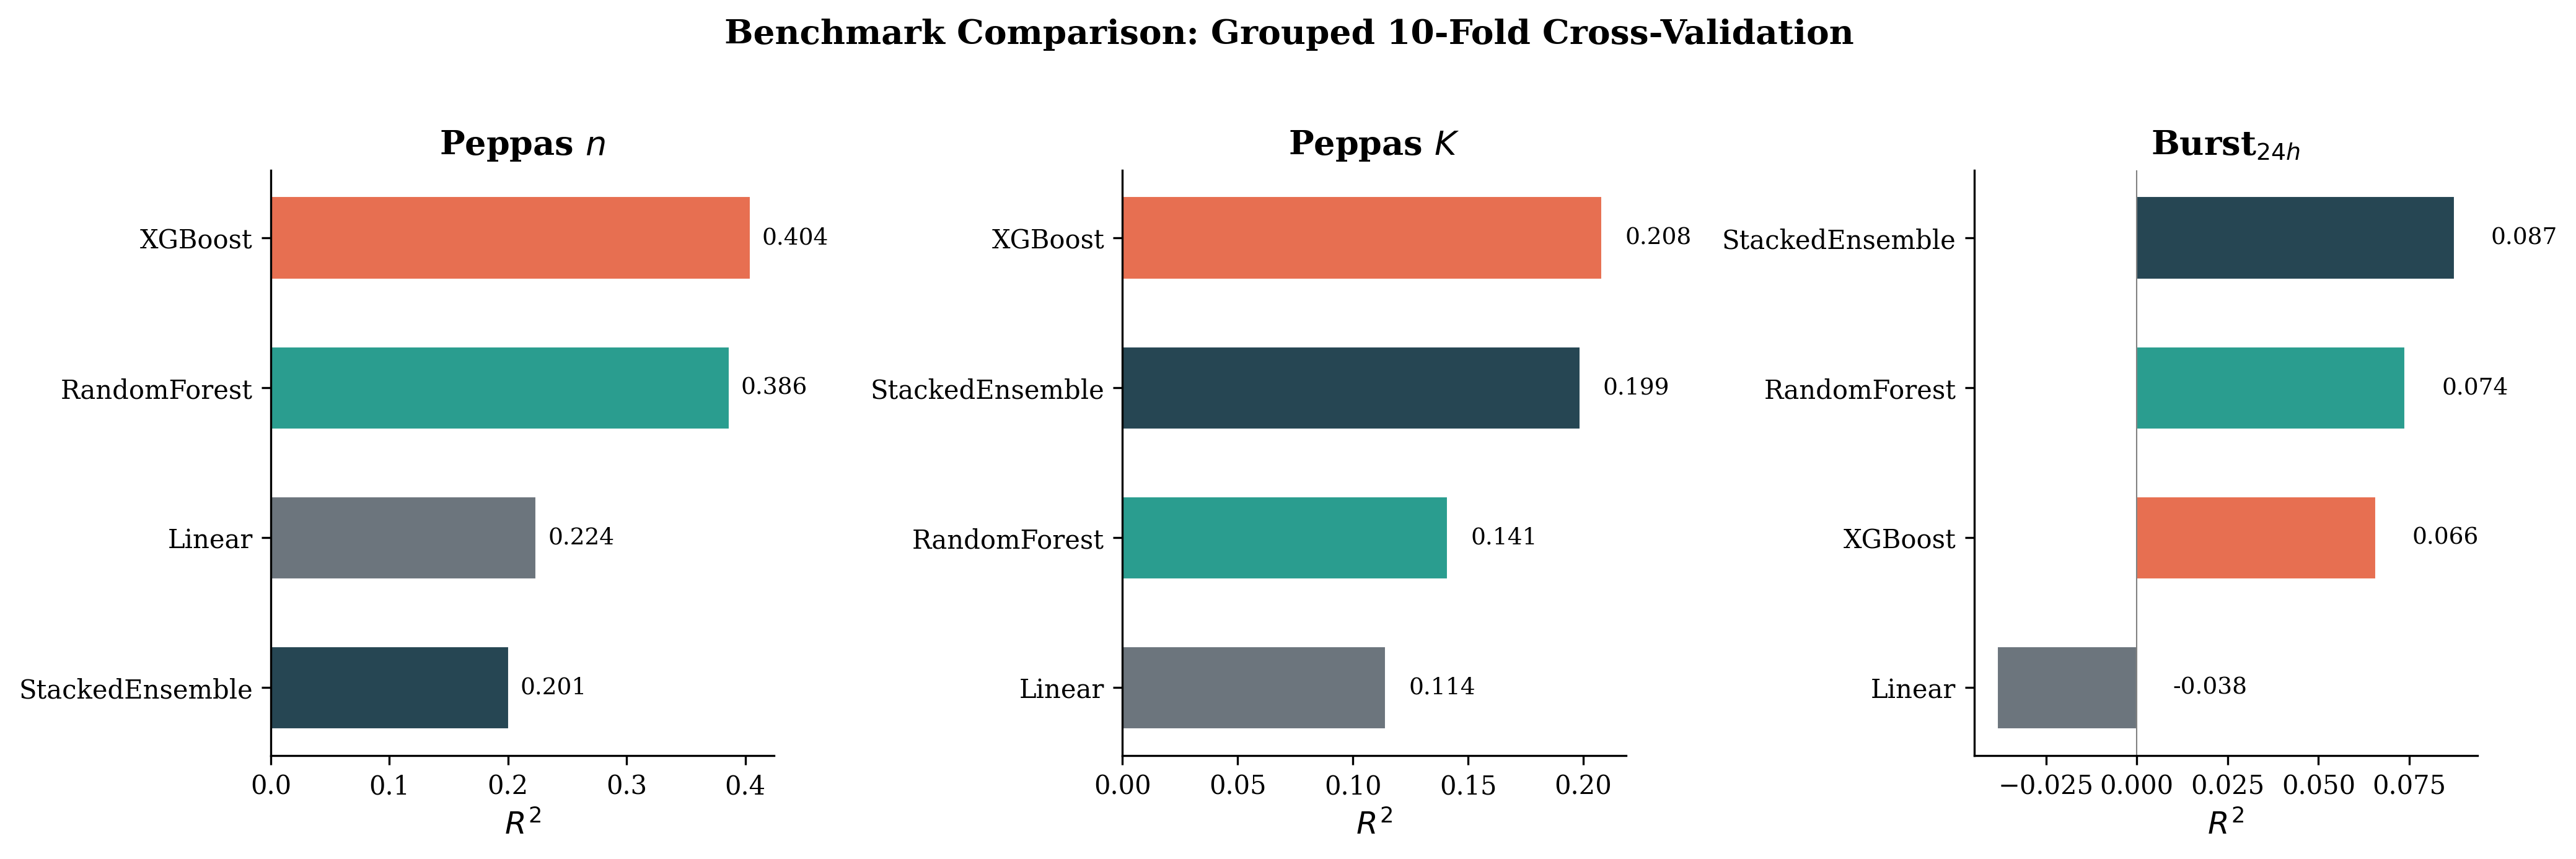
\includegraphics[width=\linewidth]{figures/fig1_benchmark_bar}
\caption{Benchmarking results for the release exponent $n$ and rate constant $K$ under grouped cross-validation.}
\label{fig:bench_bar}
\end{figure}

\FloatBarrier

% ============================================================
% 3.4  FEATURE IMPORTANCE
% ============================================================
\subsection{Feature Importance}
Feature importance for prediction of $n$ is summarized in Table~\ref{tab:feature_importance}. Polymer molecular weight contributed the largest share of importance (27.7%), followed by drug molecular weight (13.0%) and MolLogP (11.8%). A notable asymmetry exists here: the most important predictor (Polymer MW) is also one of the most frequently imputed variables (missing or unspecified in $\sim$40\% of studies), suggesting that better reporting of this single parameter could further stabilize predictions. To test whether explicit methodological details could breach the observed information ceiling, we conducted a robustness check by adding one-hot encoded formulation methods (e.g., O/W, W/O/W) as features. This yielded a negligible performance improvement ($\Delta R^2 < 0.01$), confirming that the standard physicochemical descriptors and formulation outcomes (EE, DLC) already capture the recoverable signal.

% ============================================================
% TABLE 4: Feature Importance
% ============================================================

\begin{table}[H]
\centering
\caption{Features contributing $>$5\% importance for prediction of release exponent $n$ (Random Forest).}
\label{tab:feature_importance}
\begin{tabular}{lc}
\toprule
Feature & Importance (\%) \\
\midrule
Polymer MW & 27.7 \\
Drug MW & 13.0 \\
MolLogP & 11.8 \\
LA/GA & 6.1 \\
Hydrophilicity Index & 5.9 \\
Encapsulation Eff. & 5.3 \\
\bottomrule
\end{tabular}
\end{table}

\begin{figure}[H]
\centering
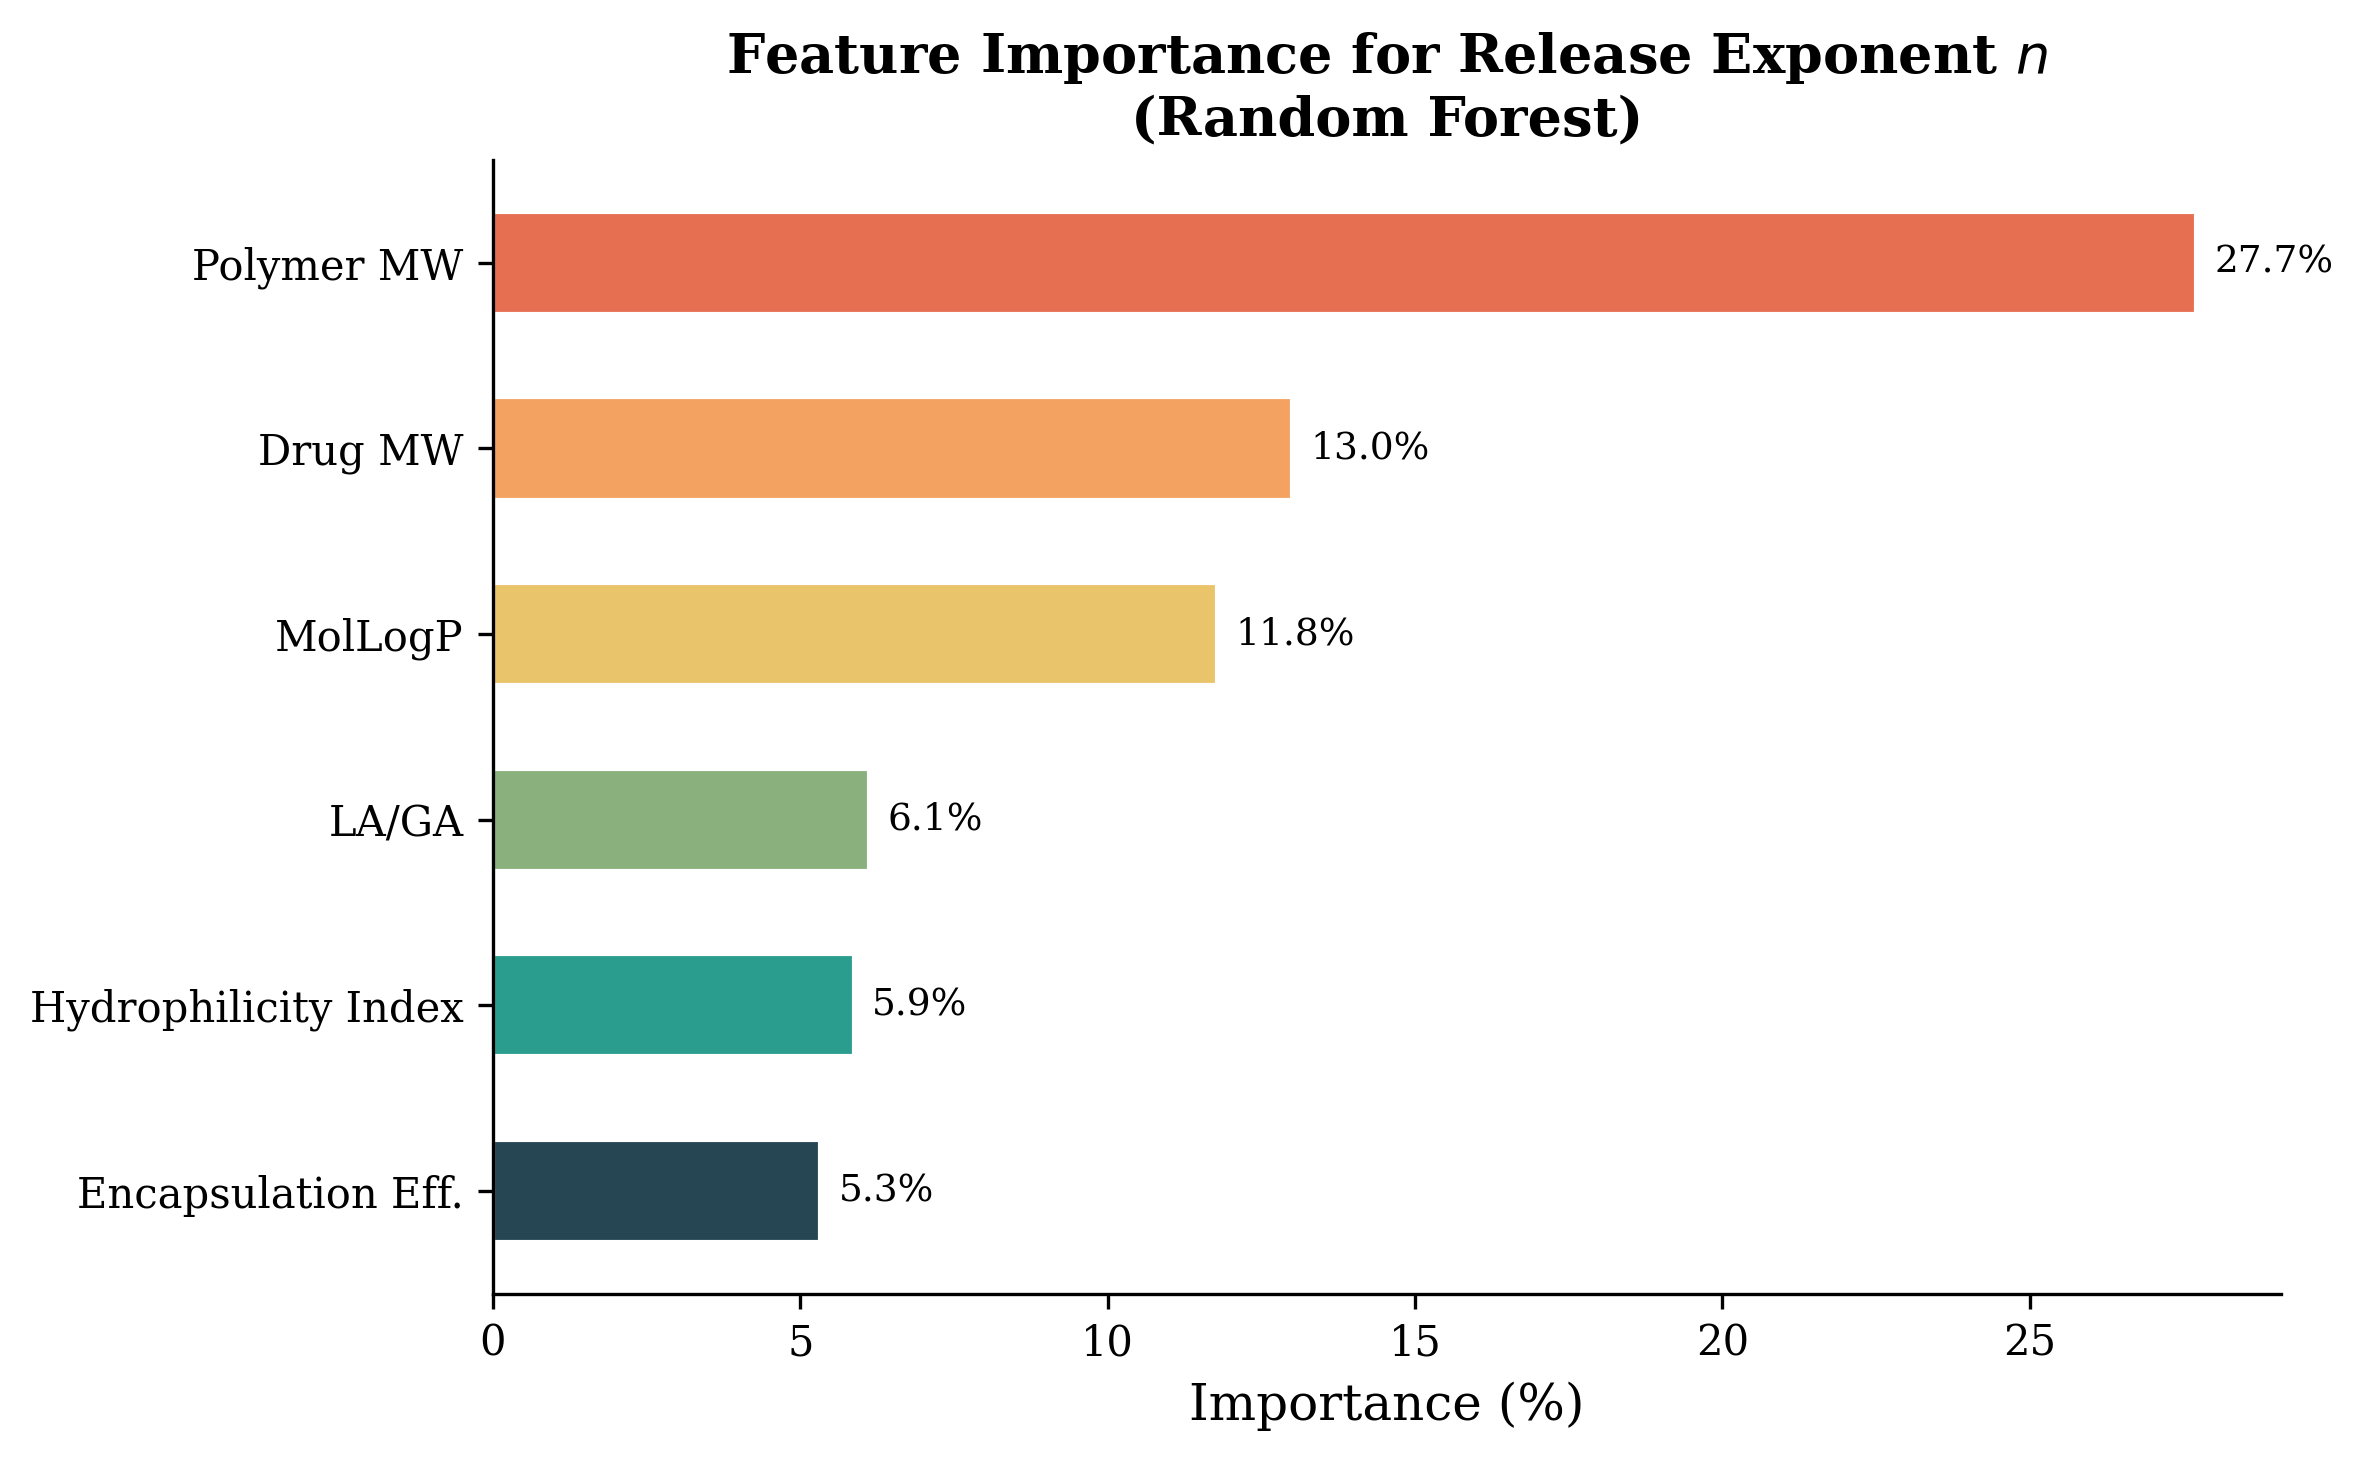
\includegraphics[width=\linewidth]{figures/fig2_feature_importance}
\caption{Top feature importances for predicting the release exponent $n$.}
\label{fig:feature_imp}
\end{figure}

\FloatBarrier

% ============================================================
% 3.5  PREDICTED VS ACTUAL
% ============================================================
\subsection{Predicted Versus Actual: Release Exponent $n$}

Predicted values for $n$ captured the overall trend but exhibited reduced dispersion relative to experimental observations. Observed $n$ values ranged from approximately 0.1 to above 1.5, whereas predictions clustered more tightly around the mean (predicted mean = 0.69, SD = 0.17 versus observed mean = 0.67, SD = 0.41).

\begin{figure}[H]
\centering
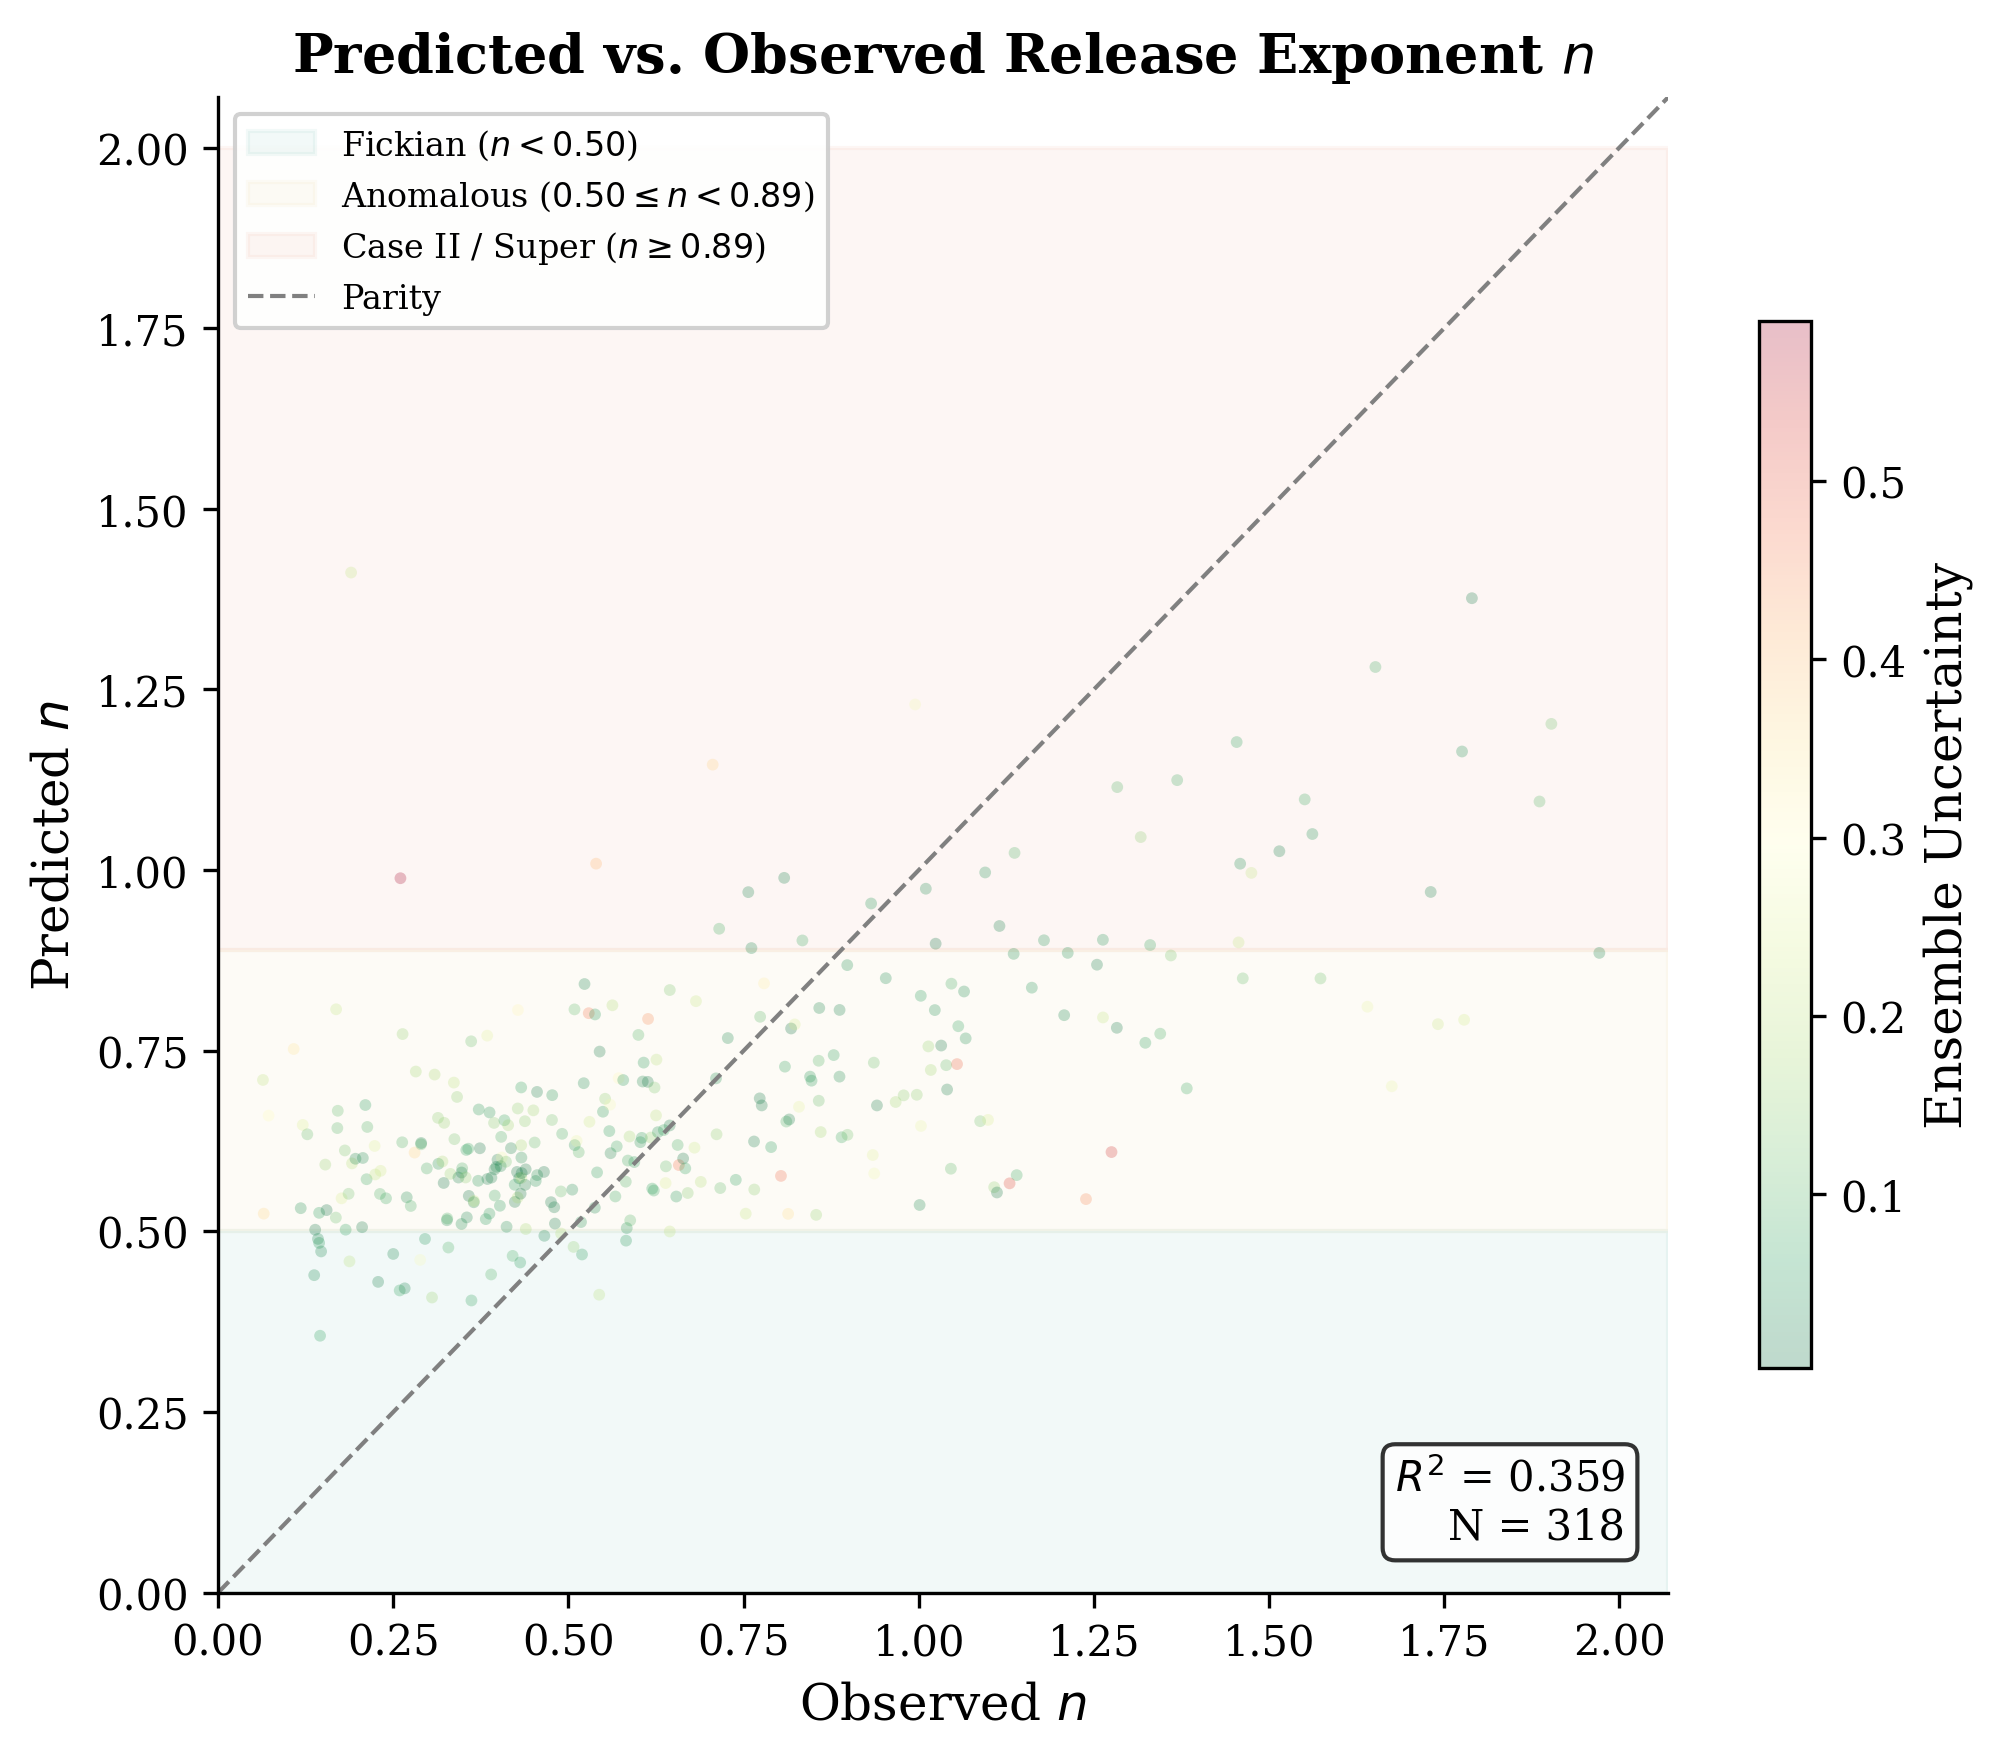
\includegraphics[width=\linewidth]{figures/fig3_pred_vs_actual_n}
\caption{Predicted versus observed release exponent $n$ (grouped cross-validation) for the modeling subset ($N = 278$ formulations). The dashed diagonal indicates parity.}
\label{fig:pred_actual_n}
\end{figure}

\FloatBarrier

% ============================================================
% 3.6  BURST RELEASE — REFRAMED AS DIAGNOSTIC FINDING
% ============================================================
\subsection{Burst Release: Regression and Classification}

\paragraph{Classification Results}
Burst release at 24 hours was the least predictable regression target ($R^2 = 0.190$). For the complementary classification task, formulations were binned into three burst-risk classes: low burst ($< 10\%$), intermediate (10--40%), and high burst ($\ge 40\%$). At the formulation level (321 unique formulations), the distribution was highly skewed: 304 formulations (94.7\%) were high burst, 15 (4.7\%) were intermediate, and 2 (0.6\%) were low burst. The confusion matrix (Table~\ref{tab:confusion_matrix}) confirmed that the model predicted only the majority class across all folds, yielding zero precision and recall for minority classes and a macro-F1 of 0.33.

\paragraph{Diagnostic Interpretation}
This distribution is itself a diagnostic finding about the published record, not a model failure. The literature as compiled reflects the typical outcome of PLGA microparticles produced under standard single or double emulsion-solvent evaporation conditions: substantial early-time release is the norm. Low-burst formulations are known to depend on microstructure-level variables---internal porosity, surface drug adsorption, solvent removal kinetics, and washing/post-processing conditions---that are rarely reported in sufficient detail to support quantitative modeling \citep{Yoo2020, Fredenberg2011}. Consequently, the extreme class imbalance (94.7\% high burst at the formulation level) renders standard classification uninformative. Standard remediation strategies---synthetic oversampling (SMOTE), cost-sensitive loss weighting, or ordinal regression---were considered but deliberately not applied. At a 95:5:1 class ratio with only 15 input features, synthetic minority generation would manufacture decision boundaries in sparsely populated regions of the feature space without genuine discriminative signal. The degeneracy is diagnostic: it reflects the absence from the literature of the process-level covariates (solvent removal rate, stirring/homogenization conditions, internal porosity) that would be needed to distinguish low-burst from high-burst formulations (Section~\ref{sec:reporting_gaps}, Table~\ref{tab:reporting_gaps}). The near-absence of low-burst formulations in the published record is itself a reporting bias that hinders the development and validation of formulation strategies yielding more controlled, clinically desirable release profiles. Until the literature systematically reports these process-level drivers, burst classification from compositional covariates alone will remain degenerate.

% ============================================================
% TABLE 6: Confusion Matrix
% ============================================================

\begin{table}[H]
\centering
\caption{Confusion matrix for three-class burst-risk classification (321 formulations). Macro-F1 = 0.33.}
\label{tab:confusion_matrix}
\begin{tabular}{lccc|c}
\toprule
 & \multicolumn{3}{c}{Predicted} & \\
\cmidrule(lr){2-4}
Actual & Low & Med & High & Recall \\
\midrule
Low ($<$10%) & 0 & 0 & 2 & 0.00 \\
Med (10--40%) & 0 & 0 & 15 & 0.00 \\
High ($\geq$40%) & 0 & 0 & 304 & 1.00 \\
\midrule
Precision & 0.00 & 0.00 & 0.95 & \\
\bottomrule
\end{tabular}
\end{table}

\FloatBarrier

% ============================================================
% 3.7  APPLICABILITY DOMAIN — EXPANDED WITH ISLAND CHARACTERIZATION
% ============================================================
\subsection{Applicability Domain Analysis}

Applicability-domain (AD) analysis was performed using leverage-based Williams plots, with warning leverage threshold $h^* = 3p/N$, where $p = 15$ is the number of features and $N$ is the number of unique formulations (the correct unit of analysis, since all targets are formulation-level quantities) \citep{Eriksson2003}. At $N = 321$ (or 318 for \texttt{Peppas\_n}, which had three formulations excluded during fitting), $h^*$ ranges from 0.141 to 0.142. Table~\ref{tab:ad_results} reports the results.

Using the correct formulation-level unit of analysis ($N = 321$), the warning leverage threshold is $h^* \approx 0.14$. Consequently, 318 of 321 formulations fall below the warning leverage for every target---only 3 high-leverage outliers are identified. The leverage values themselves (computed from the scaled design matrix) remain valid; the threshold simply reflects the appropriate sample size for formulation-level targets. This result indicates that the vast majority of the literature covers a chemically consistent design space (in-domain), yet predictive performance remains limited, reinforcing the conclusion that performance gaps are driven by unmeasured variables rather than extrapolation.

% ============================================================
% TABLE 5: AD Results
% ============================================================

\begin{table}[H]
\centering
\caption{Applicability-domain analysis: formulation-level leverage with $h^* = 3p/N$ where $N$ is the number of unique formulations.}
\label{tab:ad_results}
\begin{tabular}{llcccc}
\toprule
Target & Region & Count & $R^2$ & MAE & $h^*$ \\
\midrule
Peppas\_n & In-domain & 276 & 0.421 & 0.220 & 0.142 \\
 & High-leverage & 2 & --- & --- & \\
\midrule
Peppas\_K & In-domain & 276 & 0.272 & 0.099 & 0.140 \\
 & High-leverage & 2 & --- & --- & \\
\midrule
Burst\_24h & In-domain & 318 & 0.190 & 0.154 & 0.140 \\
 & High-leverage & 3 & --- & --- & \\
\bottomrule
\end{tabular}
\end{table}

\begin{figure}[H]
\centering
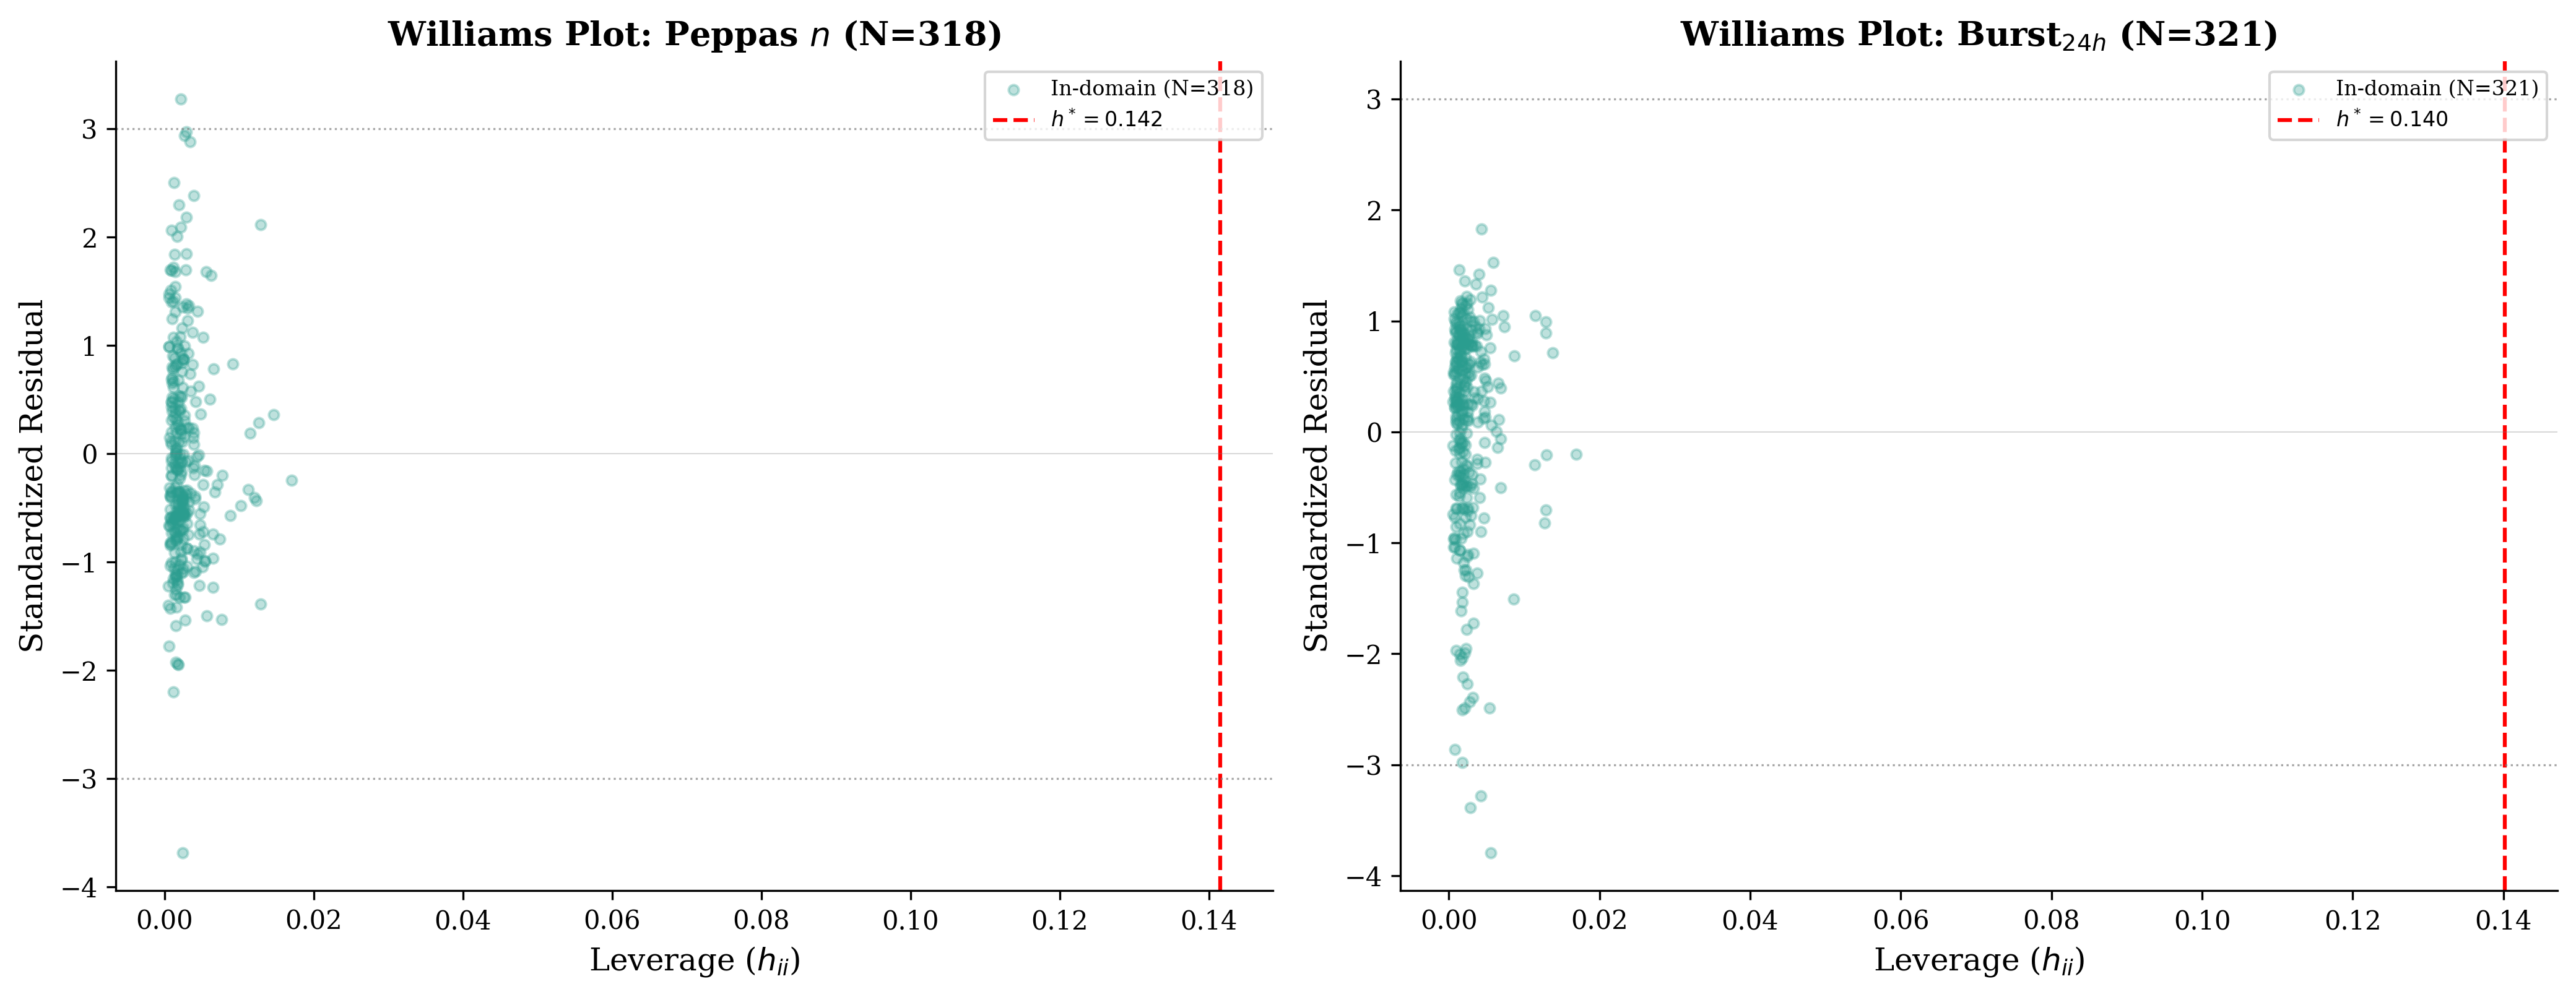
\includegraphics[width=\linewidth]{figures/fig5_williams_plot}
\caption{Williams plot for applicability-domain analysis ($N = 278$ for Peppas $n$, $N = 321$ for Burst). The vertical boundary corresponds to the warning leverage threshold $h^*$.}
\label{fig:williams}
\end{figure}

\begin{figure}[H]
\centering
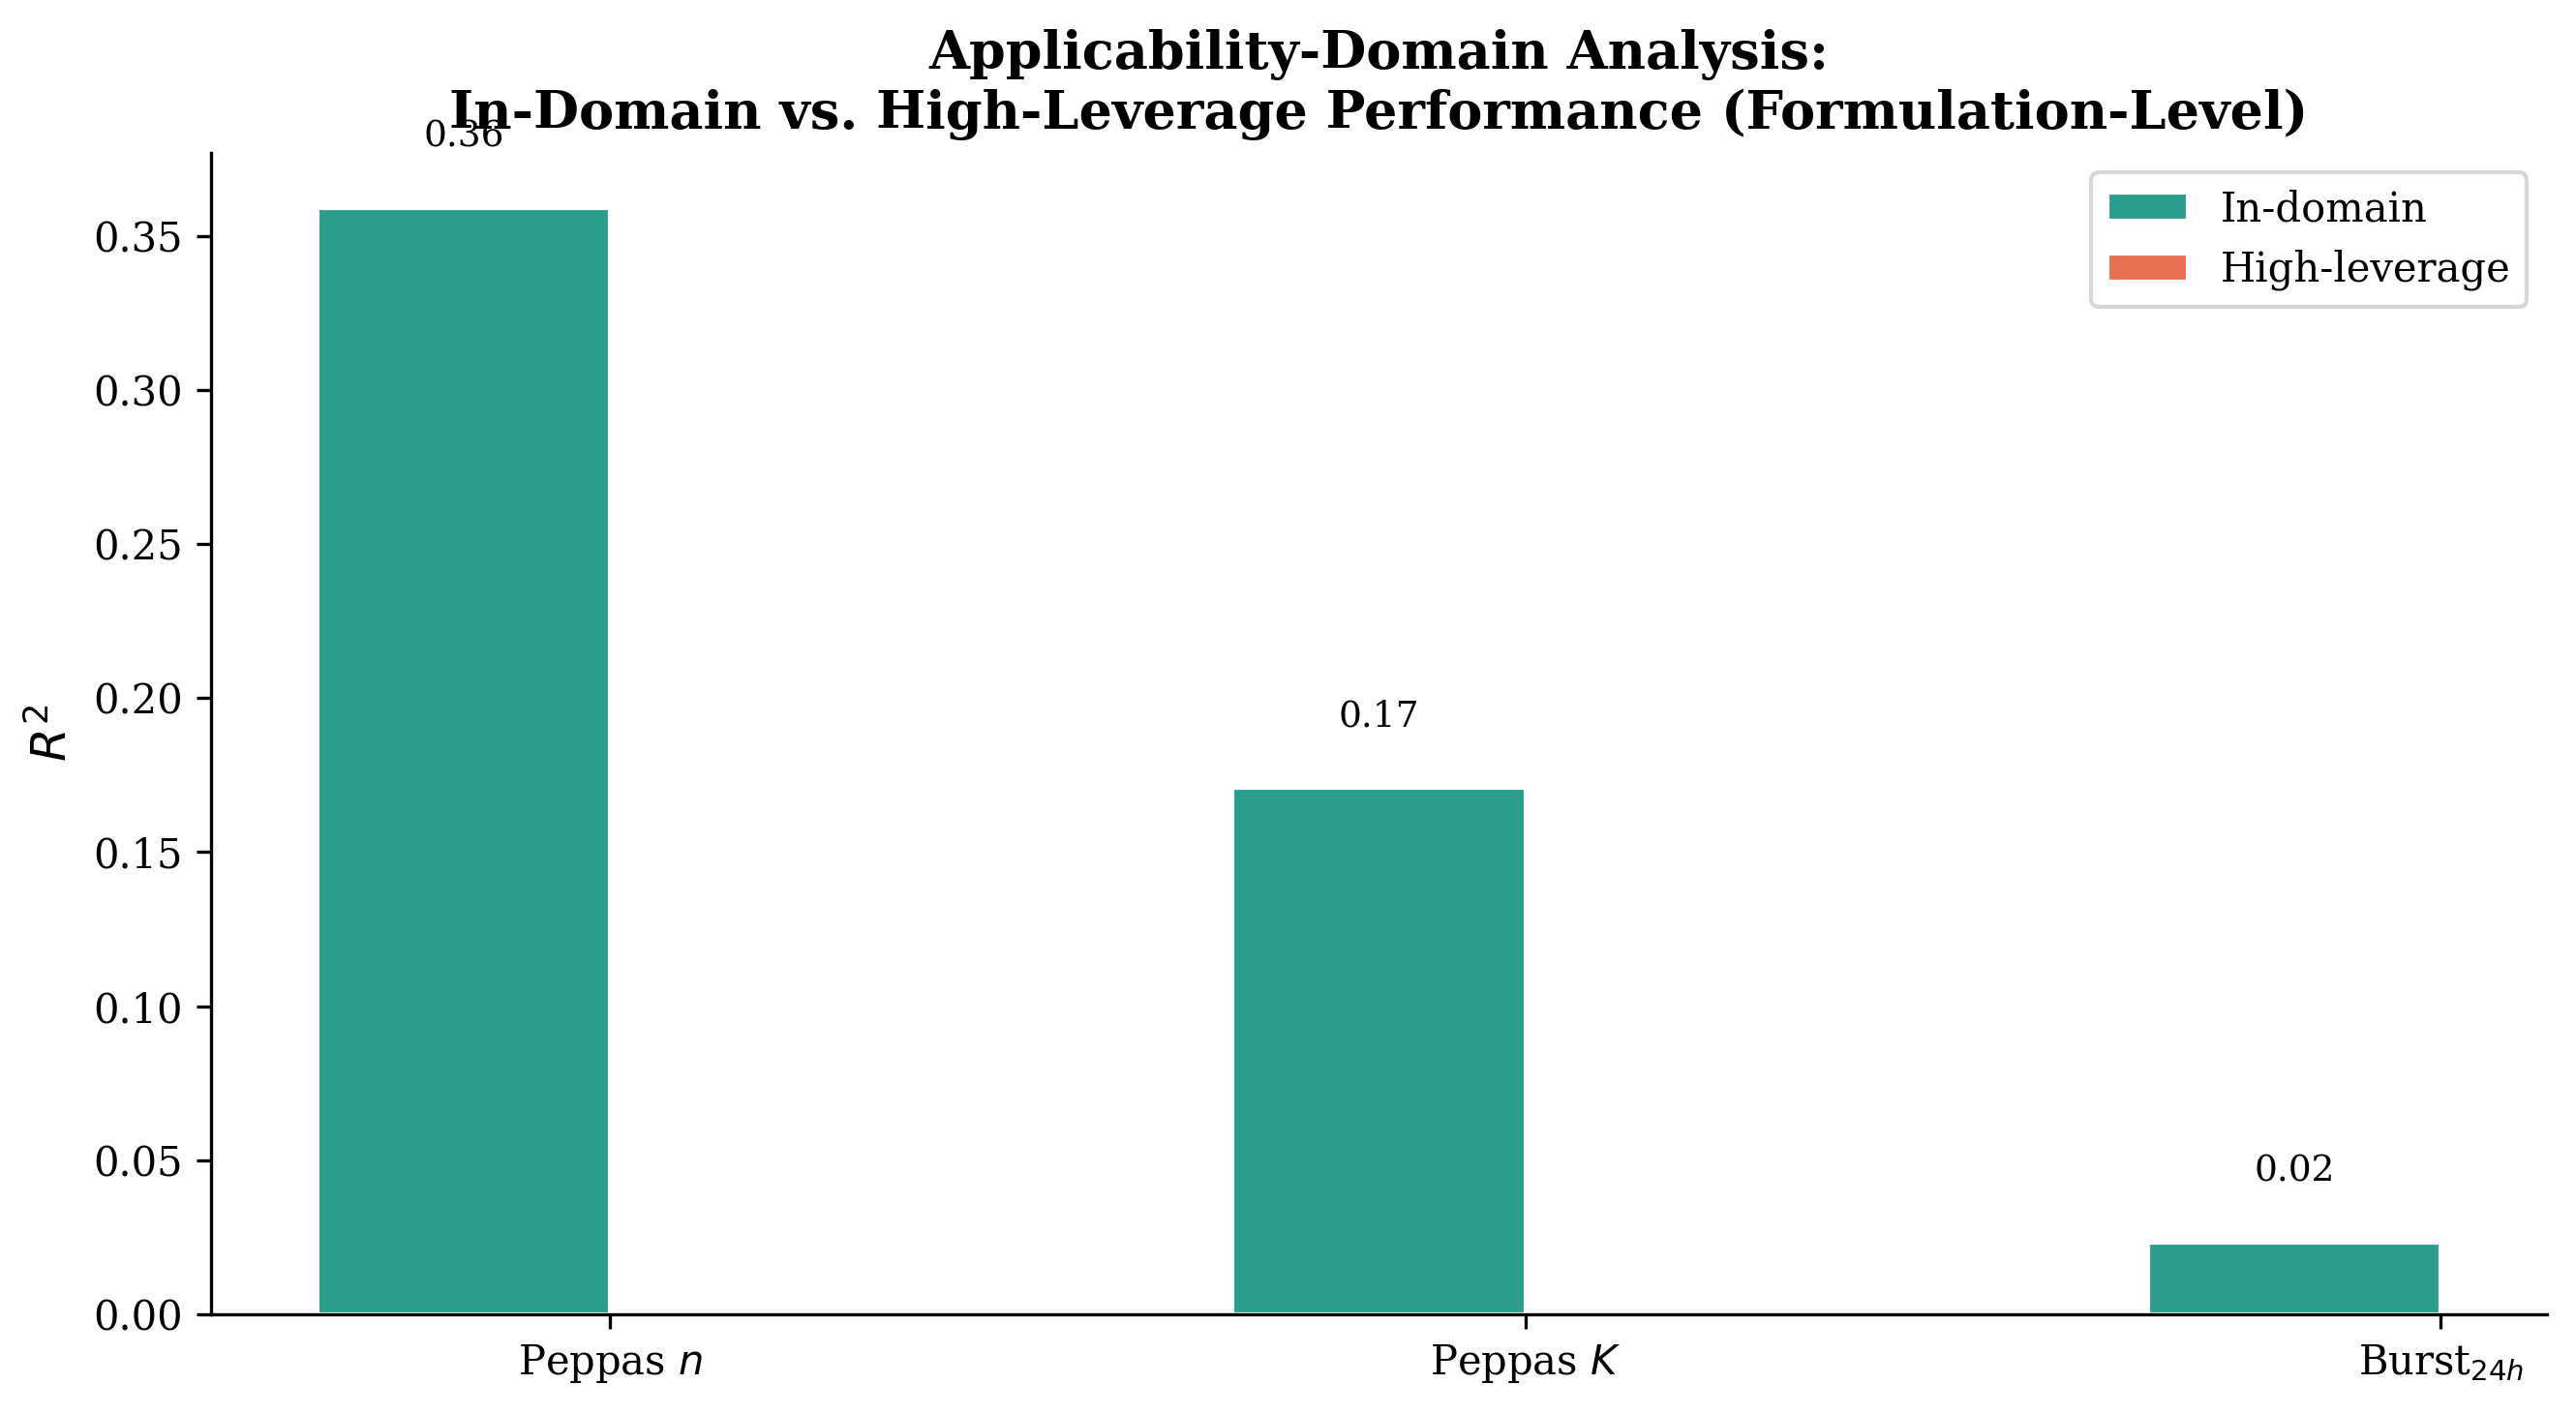
\includegraphics[width=\linewidth]{figures/fig6_ad_paradox}
\caption{Applicability-domain analysis: formulation-level $R^2$ for in-domain formulations. High-leverage formulations are extremely rare (e.g., $N=0$--3), preventing distinct performance estimation for that subgroup. With the corrected threshold ($h^* \approx 0.14$), nearly all formulations fall within the applicability domain.}
\label{fig:ad_bar}
\end{figure}



\FloatBarrier

% ============================================================
% 3.8  LOSO VALIDATION — MOVED
% ============================================================
\subsection{Leave-One-Study-Out Validation}
\label{sec:loso}

To assess the robustness of the grouped cross-validation results and test whether the observed predictive ceiling is an artifact of fold construction, leave-one-study-out (LOSO) validation was performed. In this protocol, each of the 113 unique studies (DOIs) was held out in turn, and the stacked ensemble was trained on the remaining 112 studies and evaluated on the held-out study's formulations. A cross-DOI duplicate check identified only 2 formulation pairs sharing identical features across different DOIs, confirming minimal leakage risk.

LOSO produced substantially lower pooled metrics than grouped 10-fold CV across all three targets (Table~\ref{tab:loso}). For the release exponent $n$, LOSO $R^2 = -0.083$ (MAE = 0.314), compared to grouped CV $R^2 = 0.419$ (MAE = 0.220). For $K$, LOSO $R^2 \approx 0.0$ (MAE = 0.140), and for \texttt{Burst\_24h}, LOSO $R^2 < 0$. Under leave-one-study-out validation, all targets yielded near-zero or negative $R^2$, indicating that models trained on published covariates perform worse than a na\"ive mean predictor when applied to unseen studies. The contrast with within-study grouped cross-validation---where the ensemble recovers meaningful structure ($R^2 = 0.419$ for $n$)---localizes the performance collapse to the between-study variance component. In a random-effects framework, when the majority of outcome variance is attributable to study-level random intercepts (ICC $\approx 0.66$--0.68 for $n$ and $K$; Section~\ref{sec:loso}), models trained without access to study identity are expected to degrade under LOSO validation, because the dominant variance component lies outside the modeled covariate space.

The gap between LOSO and grouped CV quantifies the magnitude of study-level confounding. Negative pooled $R^2$ across all targets indicates that inter-study variability---driven by latent, unreported process variables (solvent removal rate, homogenization energy, internal porosity)---dominates the learnable signal. The negative $R^2$ is therefore a quantitative fingerprint of the information ceiling imposed by current reporting practices.

% ============================================================
% TABLE 8: LOSO vs Grouped CV
% ============================================================

\begin{table}[H]
\centering
\caption{Comparison of grouped 10-fold CV and leave-one-study-out (LOSO) validation.}
\label{tab:loso}
\begin{tabular}{lcccccc}
\toprule
 & \multicolumn{3}{c}{Grouped 10-fold CV} & \multicolumn{3}{c}{LOSO} \\
\cmidrule(lr){2-4} \cmidrule(lr){5-7}
Target & $R^2$ & MAE & RMSE & $R^2$ & MAE & RMSE \\
\midrule
Peppas\_n & 0.419 & 0.220 & 0.292 & $-0.083$ & 0.313 & 0.404 \\
Peppas\_K & 0.272 & 0.099 & 0.155 & $-0.010$ & 0.140 & 0.177 \\
Burst\_24h & 0.190 & 0.154 & 0.411 & $-0.180$ & 0.202 & 0.245 \\
\bottomrule
\end{tabular}
\end{table}

\begin{figure}[H]
\centering
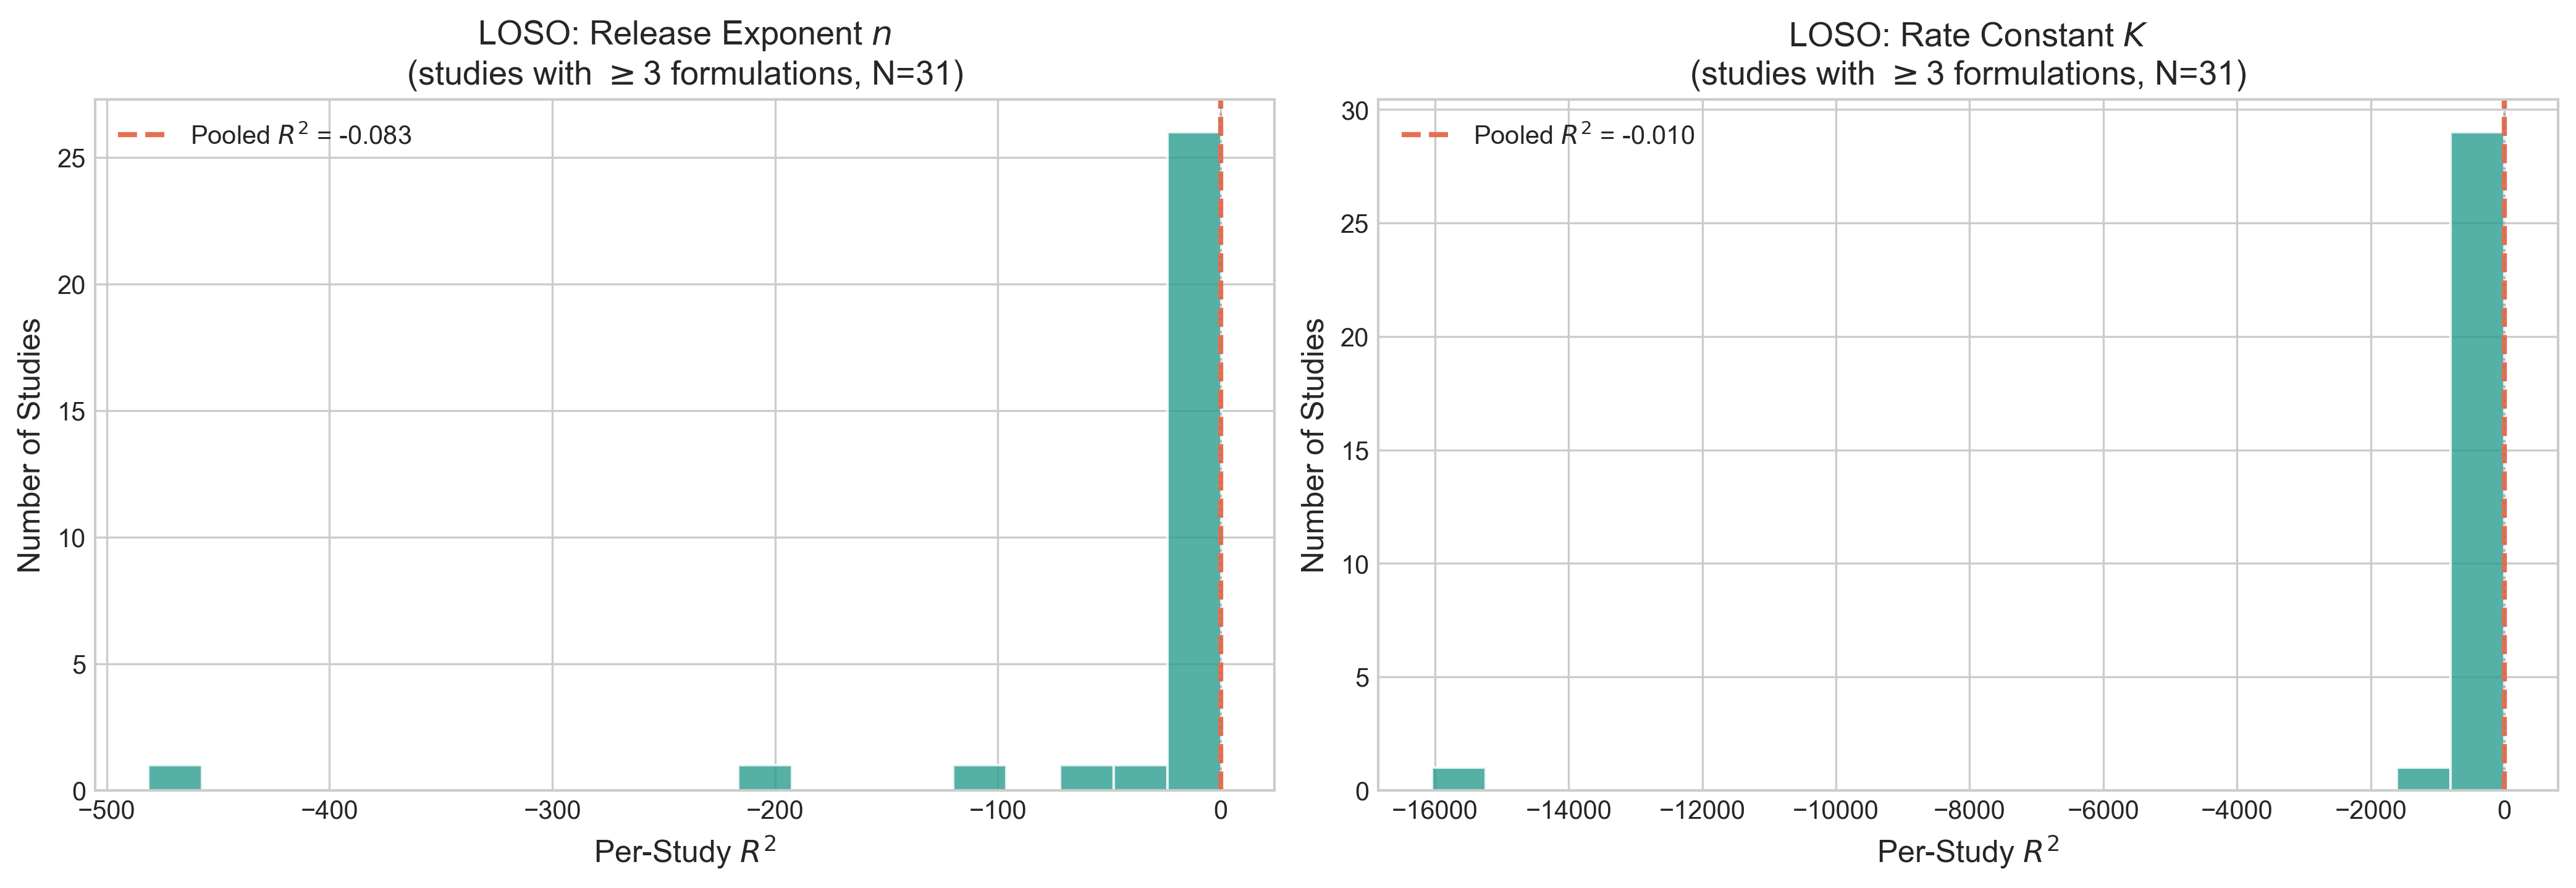
\includegraphics[width=\linewidth]{figures/fig8_loso_distribution}
\caption{Distribution of per-study $R^2$ under LOSO validation for the release exponent $n$ and rate constant $K$. Only studies contributing $\geq 3$ formulations to the held-out set are included. The pooled LOSO $R^2$ is marked as a dashed vertical line.}
\label{fig:loso_dist}
\end{figure}

\paragraph{Variance decomposition by study identity.}
To quantify the fraction of total variance attributable to study-level effects, a one-way random-effects analysis (ICC-1) was performed on the 57 studies contributing $\geq 2$ formulations (265 formulations; Table~\ref{tab:icc}). For the release exponent $n$, 67.5\% of the total variance was attributable to study identity (ICC = 0.675, $F(56, 208) = 10.55$, $p < 0.001$). For $K$, the between-study fraction was 66.0\% (ICC = 0.660), and for \texttt{Burst\_24h}, 45.9\% (ICC = 0.459); all $F$-tests were significant at $p < 0.001$. These estimates confirm that the majority of the variance in fitted release parameters originates between laboratories rather than between formulations within the same study---precisely the variance component that LOSO validation exposes and that unreported process variables are expected to generate. The lower ICC for \texttt{Burst\_24h} (0.459 vs.\ $\sim$0.67 for $n$ and $K$) is consistent with the known sensitivity of early-time release to surface microstructure and batch-level variability, which introduce substantial within-study variance even under nominally consistent protocols.

% ============================================================
% TABLE: ICC Variance Decomposition
% ============================================================

\begin{table}[H]
\centering
\caption{Variance decomposition of release parameters by study identity (ICC-1, one-way random effects model). Only studies contributing $\geq 2$ formulations are included.}
\label{tab:icc}
\begin{tabular}{lcccccc}
\toprule
Target & $k$ & $N$ & $\sigma^2_{\text{between}}$ & $\sigma^2_{\text{within}}$ & ICC(1) & $F$ ($p$-value) \\
\midrule
Peppas\_n & 57 & 265 & 0.1413 & 0.0680 & \textbf{0.675} & 10.55 ($< 0.001$) \\
Peppas\_K & 57 & 265 & 0.0246 & 0.0127 & \textbf{0.660} & 9.92 ($< 0.001$) \\
Burst\_24h & 57 & 265 & 0.0228 & 0.0268 & \textbf{0.459} & 4.89 ($< 0.001$) \\
\bottomrule
\multicolumn{7}{l}{\footnotesize $k$ = number of studies with $\geq 2$ formulations; $N$ = total formulations in those studies.} \\
\end{tabular}
\end{table}

\FloatBarrier

% ============================================================
% 3.9  UNCERTAINTY — REORDERED
% ============================================================
\subsection{Uncertainty Quantification}

Prediction uncertainty was quantified using the standard deviation of base-learner predictions within each fold. For the release exponent $n$, ensemble disagreement correlated positively with absolute prediction error (Pearson $r = 0.191$). The mean uncertainty score was 0.113 (SD = 0.108), indicating a weak but directionally useful reliability signal.

\begin{figure}[H]
\centering
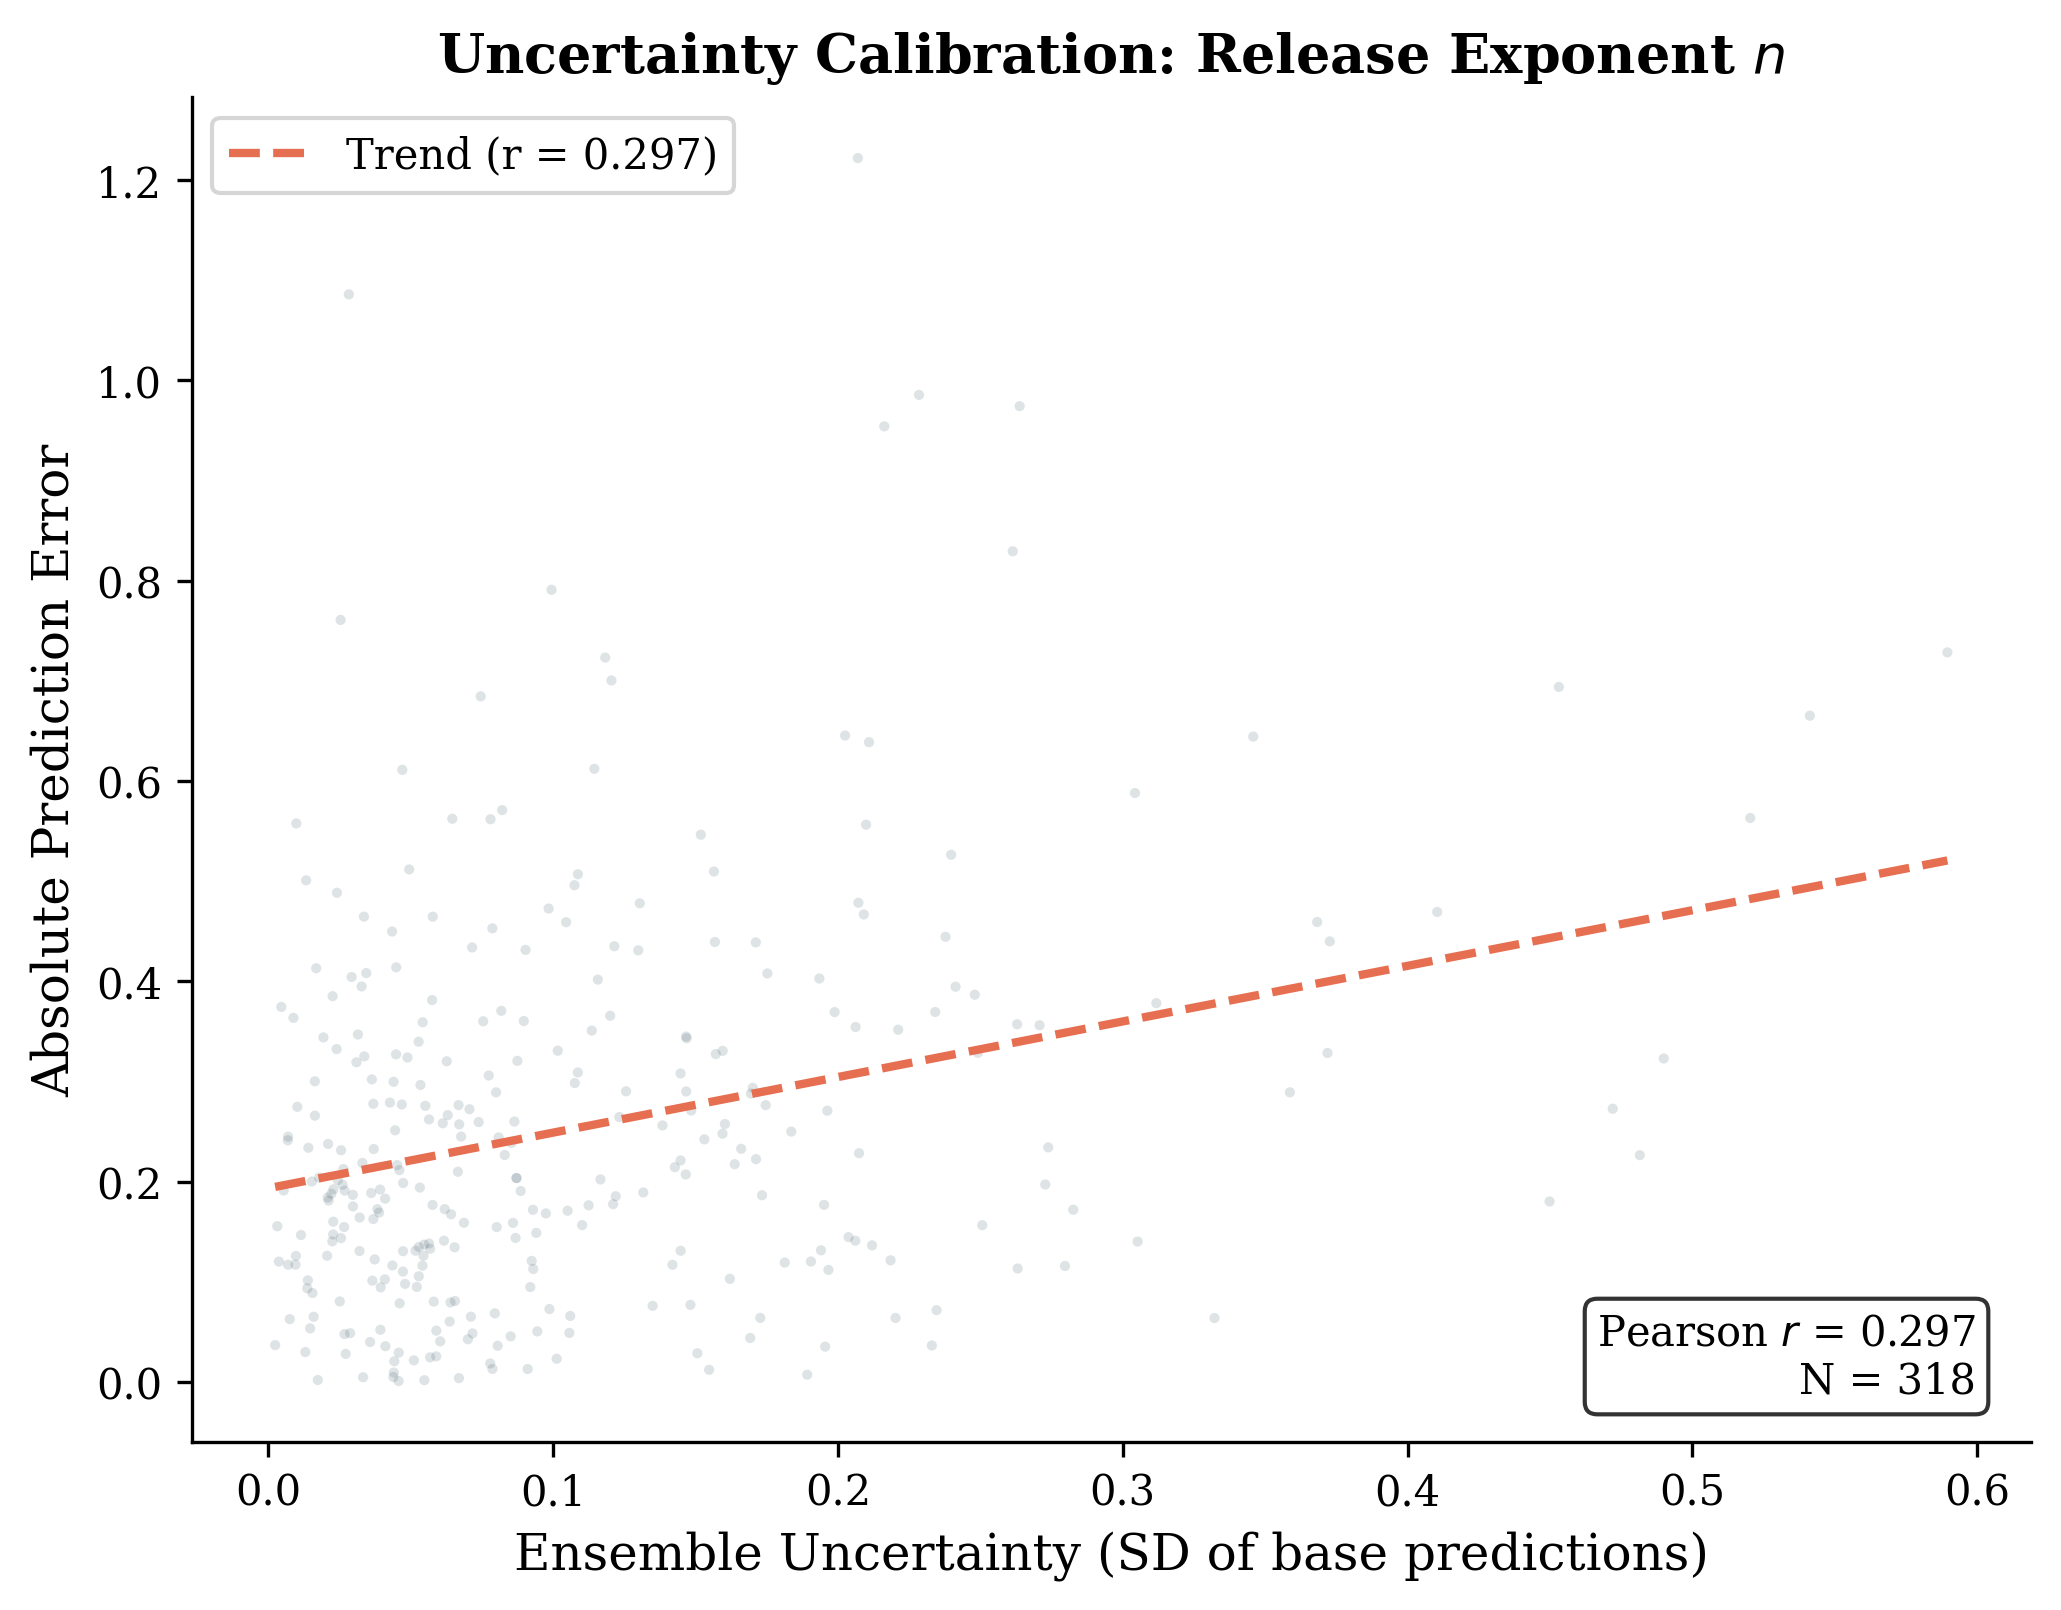
\includegraphics[width=\linewidth]{figures/fig7_uncertainty_calibration}
\caption{Uncertainty calibration for the release exponent $n$: ensemble disagreement versus absolute prediction error.}
\label{fig:uncertainty_plot}
\end{figure}

\FloatBarrier



% ============================================================
% 3.10  REPORTING GAP ANALYSIS — NEW SECTION
% ============================================================
\subsection{Reporting Gap Analysis}
\label{sec:reporting_gaps}

Table~\ref{tab:reporting_gaps} cross-references variable availability with predictive importance and mechanistic relevance. Polymer molecular weight---the dominant predictor (27.7\% importance)---was reported in a standardized form ($M_w$) by 59\% of studies. Many studies instead reported an unspecified ``molecular weight'' value without distinguishing $M_w$ from $M_n$, and a small fraction reported only $M_n$. Because these reporting categories overlap across studies (some report both $M_w$ and an unspecified MW elsewhere), we summarize availability at the formulation level: after harmonization (priority: $M_w > M_n >$ unspecified), a usable numeric polymer MW feature could be constructed for 64\% of formulations; the remaining cases required imputation. Critical polymer descriptors---$M_n$ (reported in 5\% of studies) and polydispersity index (PDI, reported in 4\%)---were too sparse to include in the model matrix despite their established roles in controlling chain-end density and molecular weight distribution breadth, both of which influence degradation kinetics and pore formation. Formulation method (O/W, S/O/W, W/O/W) was universally reported but was excluded from the numeric feature matrix to preserve a consistent numerical design space for leverage-based applicability domain calculations; exploratory models incorporating one-hot-encoded method indicators did not materially improve cross-validated performance ($\Delta R^2 < 0.01$ for all targets), suggesting that method effects are largely confounded with the continuous covariates already present.

Below these partially reported variables, Table~\ref{tab:reporting_gaps} lists four mechanistically important process-level variables that are never or almost never quantified in the source literature: internal porosity, solvent removal rate, stirring/homogenization parameters, and polymer end-group chemistry. For end-group chemistry specifically, some information might in principle be recovered from polymer trade names (e.g., the ``H'' suffix in Resomer~RG~502H denotes acid-terminated chains); however, grade-level identifiers were inconsistently reported, and no systematic rescue of end-group data was achievable across the 113 studies compiled here. These variables are known to govern early-time drug release, skin formation, and degradation pathway selection \citep{Fredenberg2011, Makadia2011}, yet their absence from the literature precludes quantitative modeling. The asymmetry between variable importance and variable reporting completeness is striking: the single most important feature (Polymer MW, 27.7\% importance) is available in standardized $M_w$ form for only 59\% of studies, while the mechanistic process variables most likely to resolve the remaining variance---internal porosity, solvent removal rate, stirring energy, end-group chemistry---are reported in 0\% of studies. This pattern directly supports the information-ceiling interpretation: the predictive ceiling is set by the reporting practices of the field rather than by algorithmic limitations.

\paragraph{Proposed minimum reporting elements (MIADR checklist)}
To enable cross-study predictive modeling, we propose the following minimum reporting standards:
\begin{itemize}
\item \textbf{Polymer Characterization:} Both $M_w$ and $M_n$ (GPC), plus polydispersity index (PDI).
\item \textbf{End-Group Chemistry:} Explicit acid-terminated vs.\ ester-capped status.
\item \textbf{Solvent Removal:} Evaporation temperature, duration, and reduced pressure conditions.
\item \textbf{Homogenization Energy:} Stirring rate (rpm), duration, and impeller/probe type.
\item \textbf{Internal Structure:} Quantitative internal porosity (e.g., via mercury porosimetry).
\end{itemize}
Adoption of these reporting elements would provide the process-level covariates needed to resolve the inter-study variance that currently dominates the noise floor, and would bring PLGA formulation reporting into closer alignment with Quality by Design (QbD) principles \citep{ICH2009}.

% ============================================================
% TABLE 7: Reporting Gaps
% ============================================================

\begin{table}[H]
\centering
\caption{Reporting gap analysis: variable availability versus predictive importance and mechanistic relevance. Variables below the mid-rule are not reported in the source literature but are known mechanistic drivers of release behavior.}
\label{tab:reporting_gaps}
\small
\begin{tabular}{llccll}
\toprule
Variable & Category & Reported (\%) & Importance (\%) & Mechanistic Role & In Model \\
\midrule
Polymer MW$^{a}$ & Polymer & 64$^{c}$ & 27.7 & Degradation rate, chain mobility & Yes (composite) \\
Polymer $M_w$ & Polymer & 59 & --- & Weight-avg MW; preferred source & Yes$^{b}$ \\
Polymer $M_n$ & Polymer & 5 & --- & Number-avg MW; chain-end density & No (94\% missing) \\
PDI & Polymer & 4 & --- & MW distribution breadth & No (96\% missing) \\
LA:GA ratio & Polymer & 100 & 6.1 & Hydrophilicity, degradation rate & Yes \\
Particle size & Formulation & 100 & 4.8 & Surface area, diffusion path & Yes \\
Drug loading & Formulation & 100 & 3.5 & Drug--polymer interaction & Yes \\
Encapsulation eff. & Formulation & 100 & 5.3 & Process efficiency proxy & Yes \\
Formulation method & Process & 100 & --- & Microstructure determinant & No (categorical) \\
Drug MW & Drug & 100 & 13.0 & Diffusivity, solubility & Yes (RDKit) \\
MolLogP & Drug & 100 & 11.8 & Lipophilicity, partitioning & Yes (RDKit) \\
\midrule
Internal porosity & Microstructure & 0 & --- & Pore-mediated diffusion & No (not reported) \\
Solvent removal rate & Process & 0 & --- & Skin formation, porosity & No (not reported) \\
Stirring/homogenization & Process & 0 & --- & Droplet size, uniformity & No (not reported) \\
End-group chemistry & Polymer & 0 & --- & Acidic vs ester end; degradation & No (not reported) \\
\bottomrule
\multicolumn{6}{l}{\footnotesize $^{a}$Composite of $M_w$, $M_n$, or unspecified MW (priority: $M_w > M_n >$ unspecified).} \\
\multicolumn{6}{l}{\footnotesize $^{b}$Contributes to composite Polymer MW when available.} \\
\multicolumn{6}{l}{\footnotesize $^{c}$Formulation-level availability after harmonization; study-level reporting categories are non-mutually exclusive.} \\
\end{tabular}
\end{table}

\FloatBarrier

% ============================================================
% LIMITATIONS (standalone section)
% ============================================================
\section{Limitations}
\label{sec:limitations}

Several limitations of this study should be acknowledged. First, release data were extracted from published figures using WebPlotDigitizer, introducing digitization noise on the order of a few percent of the ordinate value per point; this uncertainty propagates into the fitted Korsmeyer--Peppas parameters but is unlikely to account for the magnitude of inter-study variance observed. Second, protocol heterogeneity across source studies---including differences in dissolution medium (PBS vs.\ SIF), sink conditions, agitation method, and sampling frequency---represents a confound that cannot be fully disentangled from the compositional variables modeled here. Third, the attribution of the LOSO performance collapse to ``unreported process variables'' is a mechanistic interpretation supported by the reporting-gap analysis but not a proven causal relationship; unmeasured drug--polymer interactions or batch-to-batch PLGA variability may also contribute. Fourth, burst release is notoriously sensitive to surface-level microstructure---surface porosity, skin thickness, adsorbed drug layers---features that are almost never characterized in the source literature, making the negative LOSO $R^2$ for \texttt{Burst\_24h} ($-0.180$) particularly expected. Finally, the dataset is restricted to microparticles produced by emulsion-based methods and may not generalize to spray-dried, electrosprayed, or microfluidic formulations.
